\documentclass{article}
\usepackage[margin=1in]{geometry}
\usepackage{graphicx}
\usepackage{booktabs}
\usepackage{float}
\usepackage{amsmath}
\usepackage{amssymb}
\usepackage{threeparttable}
\usepackage{tikz}

\title{Project 3}
\author{Disha Dhangar, Adithya Lakshmikanth, Aastha Mishra, Ellie Truong, Amy Vu}
\date{October 2026}

\begin{document}

\maketitle

\section{2L Neural Network}
A \textbf{2-Layer Neural Network (2L)} is a basic neural network architecture consisting of an input layer and an output layer, with no hidden layers. The input layer receives the predictor variables, while the output layer generates predictions using learned weights and a bias term. Since there are no hidden layers, the model is limited to learning simple, linear relationships between the inputs and outputs.
\medskip

For this project, a 2L Neural Network is implemented using \textbf{ScalaTion} and \textbf{PyTorch} to perform regression on three datasets: Airfoil Self-Noise, Auto MPG, and Concrete Compressive Strength. The goal is to evaluate and compare the predictive performance of both implementations through hyperparameter tuning and Quality of Fit (QoF) measures, including R², MSE, and RMSE, for both in-sample and validation data.

\subsection{ScalaTion}
The ScalaTion implementation uses the built-in NeuralNet\_2L class with an identity activation function to predict numerical values across the three datasets. Each dataset was split into 80\% training and 20\% validation data, with predictors standardized using training data statistics. Hyperparameter tuning was performed by testing seven learning rates and three mini-batch sizes, selecting the combination with the lowest validation MSE. The final models were trained using ScalaTion's built-in Adam optimizer for 400 epochs and evaluated using R², MSE, and RMSE for both in-sample and validation data.
\medskip
\begin{table}[H]
    \centering
    \caption{ScalaTion 2L Neural Network Hyperparameter Tuning Results}
    \label{tab:scala_hyperparameters}
    \begin{tabular}{lccc}
        \hline
        \textbf{Dataset} & \textbf{Learning Rate} & \textbf{Batch Size} & \textbf{Validation MSE} \\
        \hline
        Airfoil  & 0.30 & 16 & 21.8925 \\
        Auto MPG & 0.30 & 16 & 12.6056 \\
        Concrete & 0.30 & 16 & 135.7732 \\
        \hline
    \end{tabular}
\end{table}

Hyperparameter tuning was performed by testing different learning rates and mini-batch sizes for each dataset. As shown in Table 1, all three datasets selected a learning rate of 0.30 and a mini-batch size of 16, as these combinations produced the lowest validation MSE among the values tested. This suggests that a higher learning rate and smaller mini-batch size were more effective for training the 2L Neural Network under the chosen settings. Because 0.30 was the largest learning rate tested, a wider range of learning rates could be explored in future work. Although the validation MSE values differ across datasets, these values should not be directly compared because each dataset predicts a different target variable with a different numerical scale.
\medskip
\begin{table}[H]
    \centering
    \caption{ScalaTion 2L Neural Network Quality of Fit Results}
    \label{tab:scala_qof}
    \small
    \begin{tabular}{lcccccc}
        \hline
        \textbf{Dataset} & \textbf{Train $R^2$} & \textbf{Validation $R^2$} & \textbf{Train MSE} & \textbf{Validation MSE} & \textbf{Train RMSE} & \textbf{Validation RMSE} \\
        \hline
        Airfoil  & 0.5214 & 0.4880 & 22.7585 & 24.2767 & 4.7706 & 4.9271 \\
        Auto MPG & 0.8248 & 0.8035 & 10.3957 & 13.0116 & 3.2242 & 3.6072 \\
        Concrete & 0.6157 & 0.6076 & 108.4138 & 104.1674 & 10.4122 & 10.2062 \\
        \hline
    \end{tabular}
\end{table}

The Quality of Fit (QoF) results were evaluated using R², MSE, and RMSE for both in-sample (training) and validation data. As shown in Table 2, Auto MPG achieved the highest validation R² of 0.8035, indicating the strongest predictive performance among the three datasets based on this metric. Concrete achieved a validation R² of 0.6076, followed by Airfoil at 0.4880. The training and validation R² values were relatively close across all three datasets, suggesting no significant signs of overfitting. Overall, the results show that the 2L Neural Network performed well on Auto MPG but had more limited predictive accuracy on Airfoil and Concrete.
\medskip
\begin{figure}[H]
    \centering

    \begin{minipage}{0.32\textwidth}
        \centering
        \includegraphics[width=\linewidth]{2L/airfoil_loss.png}
        \small (a) Airfoil
    \end{minipage}
    \hfill
    \begin{minipage}{0.32\textwidth}
        \centering
        \includegraphics[width=\linewidth]{2L/autompg_loss.png}
        \small (b) Auto MPG
    \end{minipage}
    \hfill
    \begin{minipage}{0.32\textwidth}
        \centering
        \includegraphics[width=\linewidth]{2L/concrete_loss.png}
        \small (c) Concrete
    \end{minipage}

    \caption{ScalaTion 2L Neural Network Training Loss vs. Epoch for All Three Datasets}
    \label{fig:scala_loss}
\end{figure}

Figure 1 shows the loss vs epoch plots for the Airfoil, Auto MPG, and Concrete datasets. Across all three datasets, the training loss decreases as the number of epochs increases, indicating that the neural networks are learning and reducing prediction errors. Airfoil and Auto MPG show a gradual decrease in loss before stabilizing around 250–280 epochs, while Concrete stabilizes earlier, around 150–170 epochs. Overall, the plots suggest that all three models converged during the 400 training epochs, with minimal improvement toward the end of training.
\medskip
\begin{figure}[H]
    \centering

    \begin{minipage}{0.32\textwidth}
        \centering
        \includegraphics[width=\linewidth]{2L/airfoil_actual.png}
        \small (a) Airfoil
    \end{minipage}
    \hfill
    \begin{minipage}{0.32\textwidth}
        \centering
        \includegraphics[width=\linewidth]{2L/autompg_actual.png}
        \small (b) Auto MPG
    \end{minipage}
    \hfill
    \begin{minipage}{0.32\textwidth}
        \centering
        \includegraphics[width=\linewidth]{2L/concrete_actual.png}
        \small (c) Concrete
    \end{minipage}

    \caption{ScalaTion 2L Neural Network Validation Actual vs. Predicted Values}
    \label{fig:scala_actual}
\end{figure}

Figure 2 shows the validation actual vs predicted plots for the three datasets. All three plots show a positive relationship between actual and predicted values, indicating that the models capture general trends in the data. Auto MPG shows the strongest relationship, with predictions more closely following the actual values, consistent with its higher validation R² of 0.8035. Airfoil and Concrete show greater variation between actual and predicted values, suggesting lower prediction accuracy. Overall, these plots support the Quality of Fit results and demonstrate differences in model performance across the three datasets.
\medskip
\begin{figure}[H]
    \centering

    \begin{minipage}{0.32\textwidth}
        \centering
        \includegraphics[width=\linewidth]{2L/airfoil_residual.png}
        \small (a) Airfoil
    \end{minipage}
    \hfill
    \begin{minipage}{0.32\textwidth}
        \centering
        \includegraphics[width=\linewidth]{2L/autompg_residual.png}
        \small (b) Auto MPG
    \end{minipage}
    \hfill
    \begin{minipage}{0.32\textwidth}
        \centering
        \includegraphics[width=\linewidth]{2L/concrete_residual.png}
        \small (c) Concrete
    \end{minipage}

    \caption{ScalaTion 2L Neural Network Validation Residual Plots}
    \label{fig:scala_residual}
\end{figure}

Figure 3 shows the validation residual plots for the three datasets. The residuals are distributed above and below zero, indicating that the models both overestimate and underestimate actual values. Auto MPG shows a relatively smaller spread of residuals, consistent with its lower RMSE, while Airfoil and Concrete show greater variation and noticeable patterns in their prediction errors. Overall, the residual plots suggest that the models capture general trends but may struggle with more complex relationships in the data.
\medskip

Overall, ScalaTion  produced reasonable results for a 2L Neural Network across all three datasets, with Auto MPG showing the strongest predictive performance. Interestingly, Auto MPG had the fewest observations but achieved the highest validation R², while Airfoil had the most observations but the lowest validation R². This suggests that model performance depends not only on dataset size but also on the relationships between the predictor variables and the target values. Since the 2L Neural Network has no hidden layers, it may struggle to capture more complex patterns in the Airfoil and Concrete datasets. Overall, the results demonstrate that a simple neural network can perform well on certain datasets but may be limited when relationships are more complex.


\subsection{PyTorch}
The PyTorch implementation uses a 2L Neural Network with an input layer and an output layer, with no hidden layers, to predict numerical values across the three datasets. Each dataset was split into 80\% training and 20\% validation data, with predictors standardized using training data statistics. Hyperparameter tuning was performed by testing seven learning rates and three mini-batch sizes, selecting the combination with the lowest validation MSE. Each configuration was trained using the Adam optimizer for a maximum of 100 epochs, with early stopping (patience = 10) to prevent unnecessary training, and the final model was retrained on the full training set for the best number of epochs found during tuning. Model performance was evaluated using R², MSE, and RMSE for both in-sample and validation data.
\medskip
\begin{table}[H]
    \centering
    \caption{PyTorch 2L Neural Network Hyperparameter Tuning Results}
    \label{tab:pytorch_hyperparameters}
    \small
    \begin{tabular}{lccccc}
        \hline
        \textbf{Dataset} & \textbf{Learning Rate} & \textbf{Batch Size} & \textbf{Validation MSE} & \textbf{Epochs} & \textbf{Best Epoch} \\
        \hline
        Airfoil  & 0.30 & 16 & 31.5125 & 51 & 41 \\
        Auto MPG & 0.30 & 64 & 7.8051 & 55 & 45 \\
        Concrete & 0.30 & 16 & 106.1827 & 48 & 38 \\
        \hline
    \end{tabular}
\end{table}

Hyperparameter tuning was performed by testing different learning rates and mini-batch sizes for each dataset, selecting the combination with the lowest validation MSE. As shown in Table 3, all three datasets selected a learning rate of 0.30, while Airfoil and Concrete selected a batch size of 16 and Auto MPG selected a batch size of 64. Early stopping was applied with a patience of 10 epochs, resulting in training ending at epochs 51, 55, and 48, respectively. The best validation performance occurred earlier, at epochs 41, 45, and 38. These results suggest that the selected hyperparameters varied slightly across datasets and that early stopping helped prevent unnecessary training once validation performance stopped improving. As with ScalaTion, 0.30 was the largest learning rate tested.
\medskip
\begin{table}[H]
    \centering
    \caption{PyTorch 2L Neural Network Quality of Fit Results}
    \label{tab:pytorch_qof}
    \small
    \resizebox{\textwidth}{!}{
    \begin{tabular}{lcccccc}
        \hline
        \textbf{Dataset} & \textbf{Train $R^2$} & \textbf{Validation $R^2$} & \textbf{Train MSE} & \textbf{Validation MSE} & \textbf{Train RMSE} & \textbf{Validation RMSE} \\
        \hline
        Airfoil  & 0.4977 & 0.5528 & 23.5637 & 22.4060 & 4.8542 & 4.7335 \\
        Auto MPG & 0.8255 & 0.7829 & 11.0082 & 11.0810 & 3.3179 & 3.3288 \\
        Concrete & 0.6053 & 0.6236 & 112.1226 & 96.9818 & 10.5888 & 9.8479 \\
        \hline
    \end{tabular}
    }
\end{table}

The Quality of Fit (QoF) results were evaluated using R², MSE, and RMSE for both in-sample (training) and validation data. As shown in Table 4, Auto MPG achieved the highest validation R² of 0.7829, followed by Concrete at 0.6236 and Airfoil at 0.5528. The training and validation R² values were relatively close across all three datasets, suggesting no significant signs of overfitting. Interestingly, Airfoil and Concrete achieved slightly higher validation R² values than training R² values, which can occur due to differences between the training and validation datasets. Overall, the results suggest that the 2L Neural Network performed best on Auto MPG, while Airfoil and Concrete showed more moderate predictive performance.
\medskip
\begin{figure}[H]
    \centering

    \begin{minipage}{0.32\textwidth}
        \centering
        \includegraphics[width=\linewidth]{2L/airfoil_loss_py.png}
        \small (a) Airfoil
    \end{minipage}
    \hfill
    \begin{minipage}{0.32\textwidth}
        \centering
        \includegraphics[width=\linewidth]{2L/autompg_loss_py.png}
        \small (b) Auto MPG
    \end{minipage}
    \hfill
    \begin{minipage}{0.32\textwidth}
        \centering
        \includegraphics[width=\linewidth]{2L/concrete_loss_py.png}
        \small (c) Concrete
    \end{minipage}

    \caption{PyTorch 2L Neural Network Training and Validation Loss vs. Epoch}
    \label{fig:pytorch_loss}
\end{figure}

Figure 4 shows the training and validation loss vs epoch plots for the Airfoil, Auto MPG, and Concrete datasets. Across all three datasets, the training and validation losses decrease as the number of epochs increases, indicating that the models are learning and reducing prediction errors. Airfoil shows a rapid decrease in loss before stabilizing around 10–15 epochs, while Auto MPG decreases more gradually and stabilizes around 25–30 epochs. Concrete shows a sharp initial decrease followed by small fluctuations in loss. Overall, the training and validation curves remain relatively close across all three datasets, suggesting that the models converged without significant signs of overfitting. Early stopping also helped prevent unnecessary training once validation performance stopped improving.
\medskip
\begin{figure}[H]
    \centering

    \begin{minipage}{0.32\textwidth}
        \centering
        \includegraphics[width=\linewidth]{2L/airfoil_actual_py.png}
        \small (a) Airfoil
    \end{minipage}
    \hfill
    \begin{minipage}{0.32\textwidth}
        \centering
        \includegraphics[width=\linewidth]{2L/autompg_actual_py.png}
        \small (b) Auto MPG
    \end{minipage}
    \hfill
    \begin{minipage}{0.32\textwidth}
        \centering
        \includegraphics[width=\linewidth]{2L/concrete_actual_py.png}
        \small (c) Concrete
    \end{minipage}

    \caption{PyTorch 2L Neural Network Validation Actual vs. Predicted Values}
    \label{fig:pytorch_actual}
\end{figure}

Figure 5 shows the validation actual vs predicted plots for the three datasets. The red dashed diagonal line represents perfect predictions, where predicted values equal actual values. All three datasets show a positive relationship between actual and predicted values, indicating that the models capture general trends in the data. Auto MPG shows the strongest relationship, with points generally closer to the diagonal line, consistent with its higher validation R² of 0.7829. Airfoil and Concrete show greater variation around the line, indicating less accurate predictions. Overall, these plots support the Quality of Fit results and demonstrate that the 2L Neural Network performs differently depending on the dataset.
\medskip
\begin{figure}[H]
    \centering

    \begin{minipage}{0.32\textwidth}
        \centering
        \includegraphics[width=\linewidth]{2L/airfoil_residual_py.png}
        \small (a) Airfoil
    \end{minipage}
    \hfill
    \begin{minipage}{0.32\textwidth}
        \centering
        \includegraphics[width=\linewidth]{2L/autompg_residual_py.png}
        \small (b) Auto MPG
    \end{minipage}
    \hfill
    \begin{minipage}{0.32\textwidth}
        \centering
        \includegraphics[width=\linewidth]{2L/concrete_residual_py.png}
        \small (c) Concrete
    \end{minipage}

    \caption{PyTorch 2L Neural Network Validation Residual Plots}
    \label{fig:pytorch_residual}
\end{figure}

Figure 6 shows the validation residual plots for the three datasets. The red dashed horizontal line represents zero prediction error, with points above and below the line indicating underestimation and overestimation, respectively. Airfoil shows residuals scattered around zero with some noticeable variation, while Auto MPG shows a curved pattern, suggesting that the model may not fully capture certain relationships in the data. Concrete shows a wider spread of residuals, particularly at higher predicted values, indicating greater prediction uncertainty in those ranges. Overall, the plots suggest that the models capture general trends but have limitations when predicting more complex relationships.
\medskip

Overall, PyTorch produced reasonable results for a  2L Neural Network across all three datasets, with Auto MPG achieving the highest validation R² of 0.7829. Interestingly, Auto MPG had the fewest observations but performed better than Airfoil and Concrete. This suggests that having more data does not always lead to better predictions, as performance also depends on the relationships between the input features and target values. Airfoil and Concrete showed moderate predictive performance, suggesting that their relationships may be more difficult for a simple neural network to capture. Since the 2L Neural Network has no hidden layers, it may struggle with more complex patterns in the data. Overall, the results show that PyTorch's 2L Neural Network can make useful predictions, but its accuracy depends on the dataset and the relationships within it.


\subsection{Conclusion}
Overall, both ScalaTion and PyTorch produced similar results when implementing the 2L Neural Network across the three datasets. Auto MPG achieved the highest validation R² in both implementations, despite having the fewest observations, suggesting that more data does not always guarantee better predictions. ScalaTion performed slightly better on Auto MPG, while PyTorch achieved higher validation R² values for Airfoil and Concrete. One important difference is that ScalaTion trained for 400 epochs, while PyTorch used a maximum of 100 epochs with early stopping (patience = 10). These different training conditions may have contributed to the differences in performance. The two implementations also used different random 80/20 splits, so their validation sets contain different observations, which may also contribute to these differences. Overall, the results show that a 2L Neural Network can make useful predictions, but its accuracy depends on the dataset and may be limited when relationships are more complex.

\section{3L Neural Network}
A \textbf{3-Layer Neural Network (3L)} adds one hidden layer between the input and output layers. The hidden layer applies a linear transformation followed by a nonlinear activation function, which allows the network to learn nonlinear relationships between the predictor variables and the response. An identity activation function is used at the output layer because all three tasks predict continuous numerical responses.
\medskip

For this project, a 3L Neural Network is implemented using \textbf{ScalaTion} and \textbf{PyTorch} to perform regression on the Airfoil Self-Noise, Auto MPG, and Concrete Compressive Strength datasets, and the results are evaluated using R², MSE, and RMSE for both in-sample and validation data.

\subsection{ScalaTion}

\subsubsection{Methodology}
A three-layer neural network (3L) was implemented using ScalaTion's built-in NeuralNet\_3L class to perform regression on the Airfoil Self-Noise, Auto MPG, and Concrete Compressive Strength datasets. Each network consisted of an input layer, one hidden layer, and an output layer. The number of hidden nodes, hidden-layer activation function, learning rate, and mini-batch size were tuned to identify a configuration with low validation error. An identity activation function was used at the output layer because all three tasks predict continuous numerical responses.
\medskip

The input features were standardized using the means and standard deviations calculated from the corresponding training data. The same scaling parameters were applied to the associated validation data. Each dataset was divided into an outer 80/20 training-validation split. Hyperparameter selection was conducted using an additional validation split within the outer training portion, keeping the final held-out validation data separate from hyperparameter selection.
\medskip

The hyperparameter search evaluated 36 configurations per dataset. The search considered 8, 16, and 32 hidden nodes; sigmoid and hyperbolic tangent (tanh) activation functions; learning rates of 0.01, 0.05, and 0.1; and mini-batch sizes of 32 and 64. The configuration with the lowest inner-validation mean squared error (MSE) was selected for each dataset. The final model was then trained using the selected configuration on the outer training set and evaluated on the held-out validation set.

\subsubsection{Hyperparameter-Tuning Results}
Table \ref{tab:scala3l_hyperparameters} summarizes the selected hyperparameters for each dataset.
\begin{table}[H]
    \centering
    \caption{ScalaTion 3L Neural Network Hyperparameter Tuning Results}
    \label{tab:scala3l_hyperparameters}
    \small
    \begin{tabular}{lccccc}
        \hline
        \textbf{Dataset} & \textbf{Hidden Nodes} & \textbf{Activation} & \textbf{Learning Rate} & \textbf{Batch Size} & \textbf{Inner-Validation MSE} \\
        \hline
        Airfoil  & 32 & tanh    & 0.05 & 64 & 3.7436 \\
        Auto MPG & 8  & sigmoid & 0.05 & 32 & 5.3541 \\
        Concrete & 16 & tanh    & 0.01 & 64 & 25.4735 \\
        \hline
    \end{tabular}
\end{table}

The selected configurations differed across datasets, indicating that a single set of hyperparameters was not optimal for all three regression tasks. Airfoil selected the largest hidden layer tested, whereas Auto MPG selected the smallest. Concrete selected 16 hidden nodes and a learning rate of 0.01. These results represent the best configurations within the tested search grid, rather than necessarily globally optimal settings.

\subsubsection{Quality of Fit}
The final models were evaluated using the coefficient of determination (R²), mean squared error (MSE), and root mean squared error (RMSE). Table \ref{tab:scala3l_qof} reports the training and held-out validation results.
\begin{table}[H]
    \centering
    \caption{ScalaTion 3L Neural Network Quality of Fit Results}
    \label{tab:scala3l_qof}
    \small
    \resizebox{\textwidth}{!}{
    \begin{tabular}{lcccccc}
        \hline
        \textbf{Dataset} & \textbf{Train $R^2$} & \textbf{Validation $R^2$} & \textbf{Train MSE} & \textbf{Validation MSE} & \textbf{Train RMSE} & \textbf{Validation RMSE} \\
        \hline
        Airfoil  & 0.9383 & 0.9287 & 2.9326 & 3.3829 & 1.7125 & 1.8393 \\
        Auto MPG & 0.9338 & 0.8479 & 3.9270 & 10.0701 & 1.9817 & 3.1733 \\
        Concrete & 0.9412 & 0.8986 & 16.5798 & 26.9118 & 4.0718 & 5.1877 \\
        \hline
    \end{tabular}
    }
\end{table}

The Airfoil model achieved the strongest validation R² (0.9287) and a validation RMSE of 1.8393. Its training and validation scores were relatively close, suggesting good generalization to the held-out observations in this split.
\medskip

The Auto MPG model achieved a validation R² of 0.8479 and a validation RMSE of 3.1733. Its training R² of 0.9338 was notably higher than its validation score, while its validation MSE was substantially higher than its training MSE. This gap suggests that the model fit the training data more closely than the held-out observations.
\medskip

The Concrete model achieved a validation R² of 0.8986 and a validation RMSE of 5.1877. Although its training R² was higher at 0.9412, its validation score remained relatively strong. The increase in validation error indicates some reduction in predictive accuracy on held-out observations.
\medskip

Overall, the 3L neural networks achieved relatively high validation R² values across the three datasets, with Airfoil showing the closest training-validation agreement and Auto MPG showing the largest generalization gap. RMSE values should be interpreted within each dataset because the response variables have different units and scales. These results describe one train-validation split and the hyperparameter grid tested; additional splits or random seeds would be needed to assess the stability of the results.

\subsubsection{Training Loss and Prediction Plots}
Figures \ref{fig:scala3l_airfoil}--\ref{fig:scala3l_concrete} show the training-loss curves and the actual-versus-predicted responses for the training and held-out validation sets. The loss curves illustrate the change in training loss over epochs, while the prediction plots allow visual assessment of the agreement between observed and predicted responses.
\medskip
\begin{figure}[H]
    \centering

    \begin{minipage}{0.32\textwidth}
        \centering
        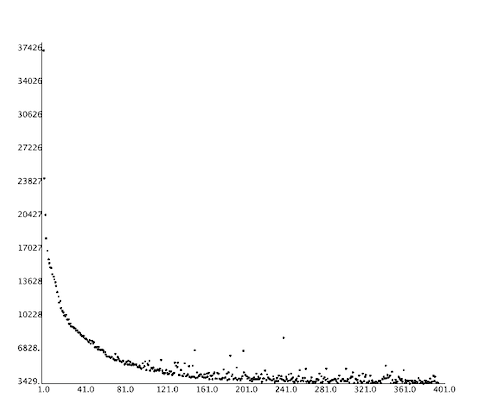
\includegraphics[width=\linewidth]{3L/scala_airfoil_loss.png}
        \small (a) Training Loss
    \end{minipage}
    \hfill
    \begin{minipage}{0.32\textwidth}
        \centering
        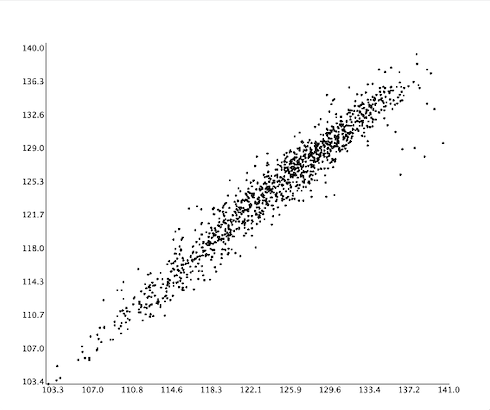
\includegraphics[width=\linewidth]{3L/scala_airfoil_train.png}
        \small (b) Training
    \end{minipage}
    \hfill
    \begin{minipage}{0.32\textwidth}
        \centering
        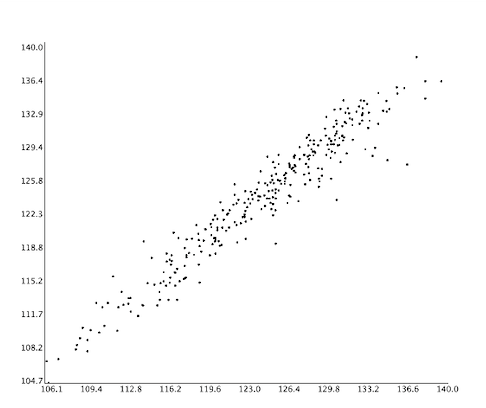
\includegraphics[width=\linewidth]{3L/scala_airfoil_val.png}
        \small (c) Validation
    \end{minipage}

    \caption{ScalaTion 3L Neural Network Results for Airfoil: Training Loss vs. Epoch and Actual vs. Predicted Values}
    \label{fig:scala3l_airfoil}
\end{figure}

\begin{figure}[H]
    \centering

    \begin{minipage}{0.32\textwidth}
        \centering
        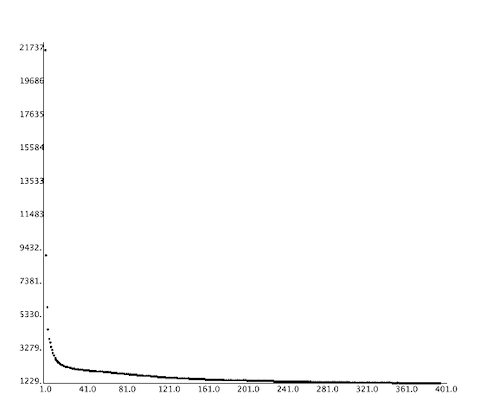
\includegraphics[width=\linewidth]{3L/scala_autompg_loss.png}
        \small (a) Training Loss
    \end{minipage}
    \hfill
    \begin{minipage}{0.32\textwidth}
        \centering
        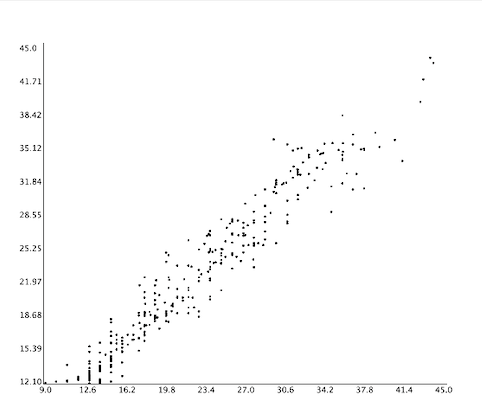
\includegraphics[width=\linewidth]{3L/scala_autompg_train.png}
        \small (b) Training
    \end{minipage}
    \hfill
    \begin{minipage}{0.32\textwidth}
        \centering
        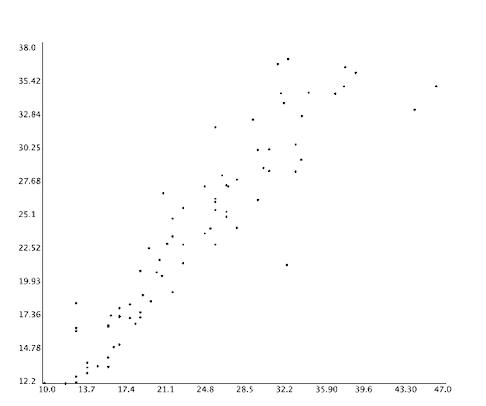
\includegraphics[width=\linewidth]{3L/scala_autompg_val.png}
        \small (c) Validation
    \end{minipage}

    \caption{ScalaTion 3L Neural Network Results for Auto MPG: Training Loss vs. Epoch and Actual vs. Predicted Values}
    \label{fig:scala3l_autompg}
\end{figure}

\begin{figure}[H]
    \centering

    \begin{minipage}{0.32\textwidth}
        \centering
        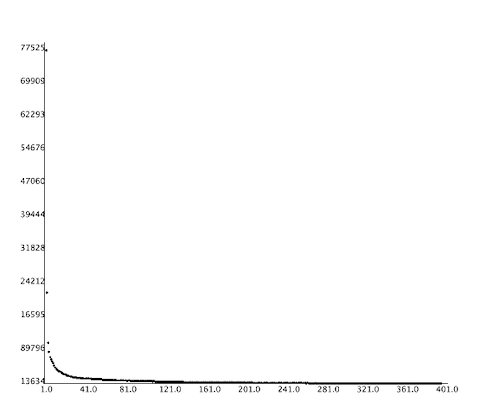
\includegraphics[width=\linewidth]{3L/scala_concrete_loss.png}
        \small (a) Training Loss
    \end{minipage}
    \hfill
    \begin{minipage}{0.32\textwidth}
        \centering
        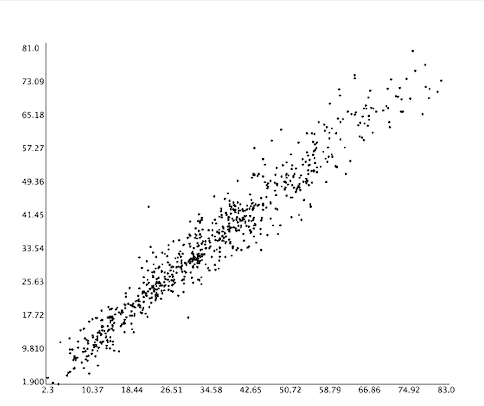
\includegraphics[width=\linewidth]{3L/scala_concrete_train.png}
        \small (b) Training
    \end{minipage}
    \hfill
    \begin{minipage}{0.32\textwidth}
        \centering
        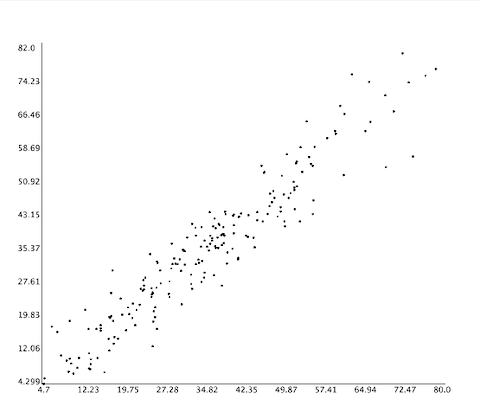
\includegraphics[width=\linewidth]{3L/scala_concrete_val.png}
        \small (c) Validation
    \end{minipage}

    \caption{ScalaTion 3L Neural Network Results for Concrete: Training Loss vs. Epoch and Actual vs. Predicted Values}
    \label{fig:scala3l_concrete}
\end{figure}

In all three datasets the training loss drops sharply during the first epochs and then levels off; Airfoil keeps decreasing gradually until roughly epoch 200, while Auto MPG and Concrete flatten out much earlier. The training and validation predictions follow the diagonal for all three datasets, with the tightest pattern for Airfoil. For Auto MPG, the validation predictions show noticeably more spread than the training predictions, consistent with its larger generalization gap in Table \ref{tab:scala3l_qof}.

\subsection{PyTorch}
The PyTorch implementation uses a three-layer (3L) neural network with an input layer, one hidden layer, and an output layer to perform regression on the Airfoil Self-Noise, Auto MPG, and Concrete Compressive Strength datasets. The output layer is a single linear (identity) node because each task predicts a continuous response. Each dataset was split into 80\% training and 20\% validation data using the same random seed as the other PyTorch models, and the predictors were standardized using the mean and standard deviation of the training data only. The same scaling was then applied to the validation data. As in the 4L and 5L models, the target variable was also standardized using the training mean and standard deviation, and predictions were converted back to the original scale before calculating the QoF measures.
\medskip

Hyperparameter tuning was carried out on the training portion only, so the final validation data remained untouched. The training data was split again into an inner 80\% training set and a 20\% inner validation set, and the scalers were refit on the inner training set. The search covered 180 configurations per dataset: 4, 8, 16, and 32 hidden nodes; ReLU, tanh, and sigmoid hidden-layer activations; learning rates of 0.001, 0.005, 0.01, 0.05, and 0.1; and mini-batch sizes of 16, 32, and 64. Every configuration was trained with the Adam optimizer and the MSE loss for at most 300 epochs, with early stopping (patience = 20) based on the inner-validation MSE. The configuration with the lowest inner-validation MSE was selected for each dataset. The final model was then retrained on the full training set using the selected configuration, for the number of epochs at which the inner-validation MSE was lowest, and evaluated using R², MSE, and RMSE on both the training and validation data.
\medskip
\begin{table}[H]
    \centering
    \caption{PyTorch 3L Neural Network Hyperparameter Tuning Results}
    \label{tab:pytorch3l_hyperparameters}
    \small
    \begin{tabular}{lcccccc}
        \hline
        \textbf{Dataset} & \textbf{Hidden Nodes} & \textbf{Activation} & \textbf{Learning Rate} & \textbf{Batch Size} & \textbf{Inner-Val. MSE} & \textbf{Best Epoch} \\
        \hline
        Airfoil  & 32 & ReLU & 0.005 & 32 & 5.5591 & 269 \\
        Auto MPG & 8  & ReLU & 0.05  & 16 & 5.6425 & 12 \\
        Concrete & 32 & tanh & 0.005 & 32 & 18.2305 & 300 \\
        \hline
    \end{tabular}
\end{table}

The selected configurations differ across the three datasets, so no single set of hyperparameters was best for every regression task. Airfoil and Concrete both selected the largest hidden layer (32 nodes) and a learning rate of 0.005, while Auto MPG, the smallest dataset, selected only 8 hidden nodes and a learning rate of 0.05. ReLU was selected for Airfoil and Auto MPG and tanh for Concrete. Airfoil and Concrete reached their best inner-validation MSE late in training (epochs 269 and 300), and Concrete reached the 300-epoch limit, which suggests that it could improve slightly with longer training. Auto MPG reached its best inner-validation MSE after only 12 epochs. These results show the configurations that minimized inner-validation MSE within the tested grid and do not establish that they are globally optimal.
\medskip
\begin{table}[H]
    \centering
    \caption{PyTorch 3L Neural Network Quality of Fit Results}
    \label{tab:pytorch3l_qof}
    \small
    \resizebox{\textwidth}{!}{
    \begin{tabular}{lcccccc}
        \hline
        \textbf{Dataset} & \textbf{Train $R^2$} & \textbf{Validation $R^2$} & \textbf{Train MSE} & \textbf{Validation MSE} & \textbf{Train RMSE} & \textbf{Validation RMSE} \\
        \hline
        Airfoil  & 0.9189 & 0.9072 & 3.8029 & 4.6483 & 1.9501 & 2.1560 \\
        Auto MPG & 0.8785 & 0.8526 & 7.6661 & 7.5248 & 2.7688 & 2.7431 \\
        Concrete & 0.9570 & 0.8923 & 12.2291 & 27.7473 & 3.4970 & 5.2676 \\
        \hline
    \end{tabular}
    }
\end{table}

The Quality of Fit (QoF) results were evaluated using R², MSE, and RMSE for both the training (in-sample) and validation data. As shown in Table \ref{tab:pytorch3l_qof}, Airfoil achieved the highest validation R² of 0.9072, followed by Concrete at 0.8923 and Auto MPG at 0.8526. Airfoil shows a small gap between training and validation R² (0.9189 versus 0.9072), which suggests the model generalized well on this split. Auto MPG also shows a small gap (0.8785 versus 0.8526), and its validation MSE is slightly lower than its training MSE. Concrete shows the largest gap: its training R² is 0.9570, but its validation MSE (27.75) is more than twice its training MSE (12.23), indicating that the model fit the training data more closely than the held-out data. RMSE values should be compared only within a dataset because the response variables have different units and scales. The inner-validation MSE in Table \ref{tab:pytorch3l_hyperparameters} should also not be compared directly with the validation MSE in Table \ref{tab:pytorch3l_qof}, since they are computed on different validation sets and, for the final model, after retraining on more data.
\medskip

To check how much these results depend on the random initialization, the final models were retrained with five different seeds. The mean validation R² values were 0.9026 ($\pm$0.0055) for Airfoil, 0.8277 ($\pm$0.0197) for Auto MPG, and 0.8746 ($\pm$0.0169) for Concrete. Airfoil is very stable, while the single-seed Auto MPG result in Table \ref{tab:pytorch3l_qof} is on the high end of its range (0.7959 to 0.8453).
\medskip
\begin{figure}[H]
    \centering

    \begin{minipage}{0.32\textwidth}
        \centering
        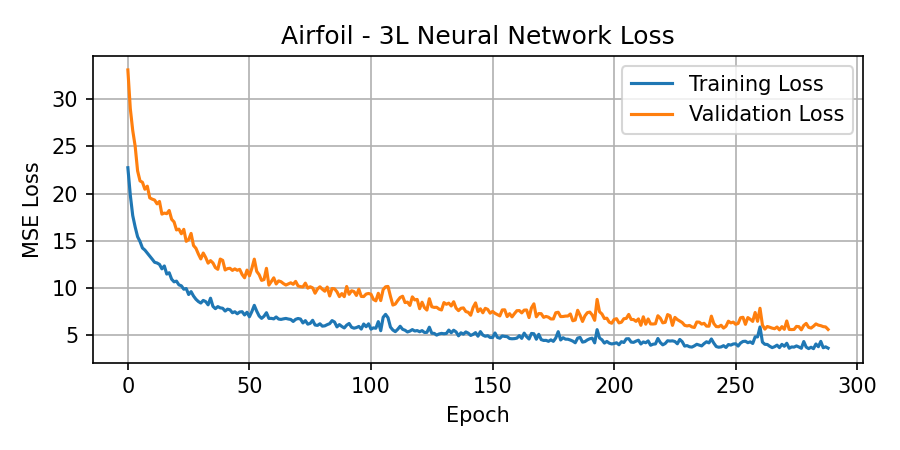
\includegraphics[width=\linewidth]{3L/pytorch_airfoil_loss.png}
        \small (a) Airfoil
    \end{minipage}
    \hfill
    \begin{minipage}{0.32\textwidth}
        \centering
        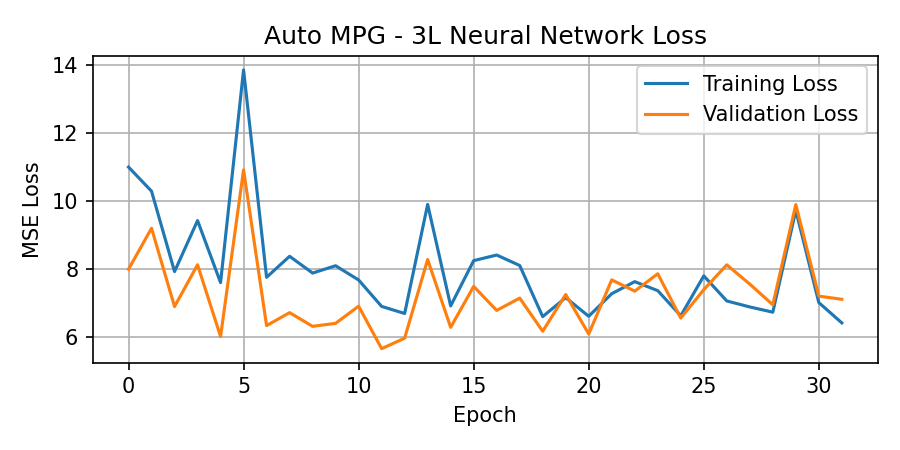
\includegraphics[width=\linewidth]{3L/pytorch_autompg_loss.png}
        \small (b) Auto MPG
    \end{minipage}
    \hfill
    \begin{minipage}{0.32\textwidth}
        \centering
        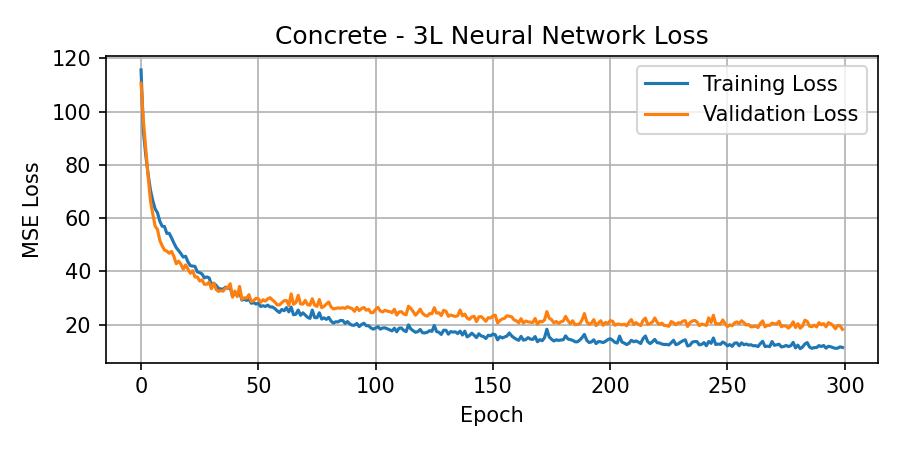
\includegraphics[width=\linewidth]{3L/pytorch_concrete_loss.png}
        \small (c) Concrete
    \end{minipage}

    \caption{PyTorch 3L Neural Network Training and Validation Loss vs. Epoch (Tuning Run, Selected Configuration)}
    \label{fig:pytorch3l_loss}
\end{figure}

Figure \ref{fig:pytorch3l_loss} shows the training and inner-validation loss versus epoch for the selected configuration of each dataset. These curves come from the tuning run, so they are computed on the inner training and inner validation sets rather than on the final models. Airfoil and Concrete drop sharply during the first few epochs and then keep decreasing slowly for the rest of the run, with the validation loss staying slightly above the training loss. Auto MPG is much noisier, with a spike near epoch 5, which reflects its high learning rate (0.05) and small number of observations; its best validation loss occurs at epoch 12.
\medskip
\begin{figure}[H]
    \centering

    \begin{minipage}{0.32\textwidth}
        \centering
        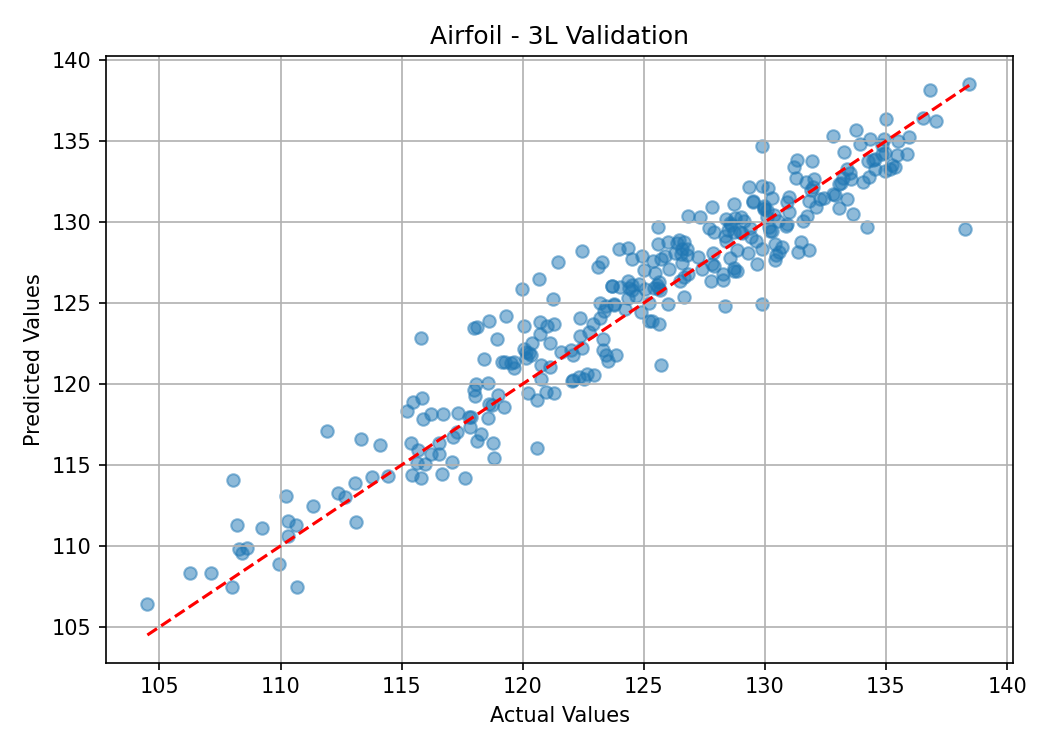
\includegraphics[width=\linewidth]{3L/pytorch_airfoil_actual.png}
        \small (a) Airfoil
    \end{minipage}
    \hfill
    \begin{minipage}{0.32\textwidth}
        \centering
        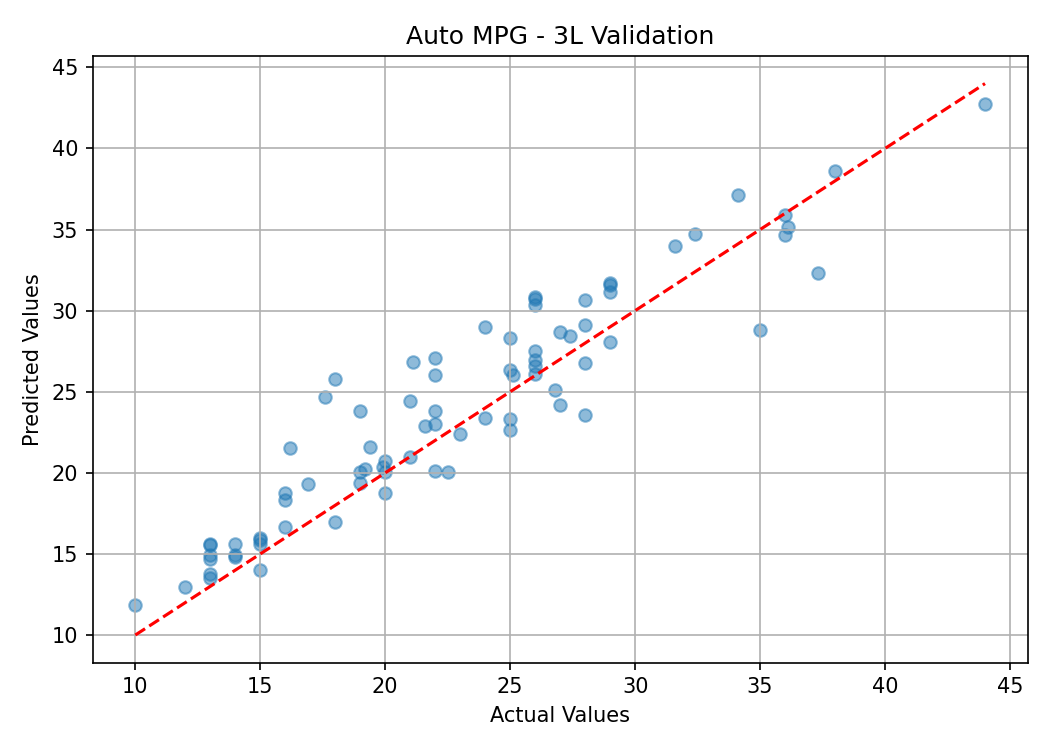
\includegraphics[width=\linewidth]{3L/pytorch_autompg_actual.png}
        \small (b) Auto MPG
    \end{minipage}
    \hfill
    \begin{minipage}{0.32\textwidth}
        \centering
        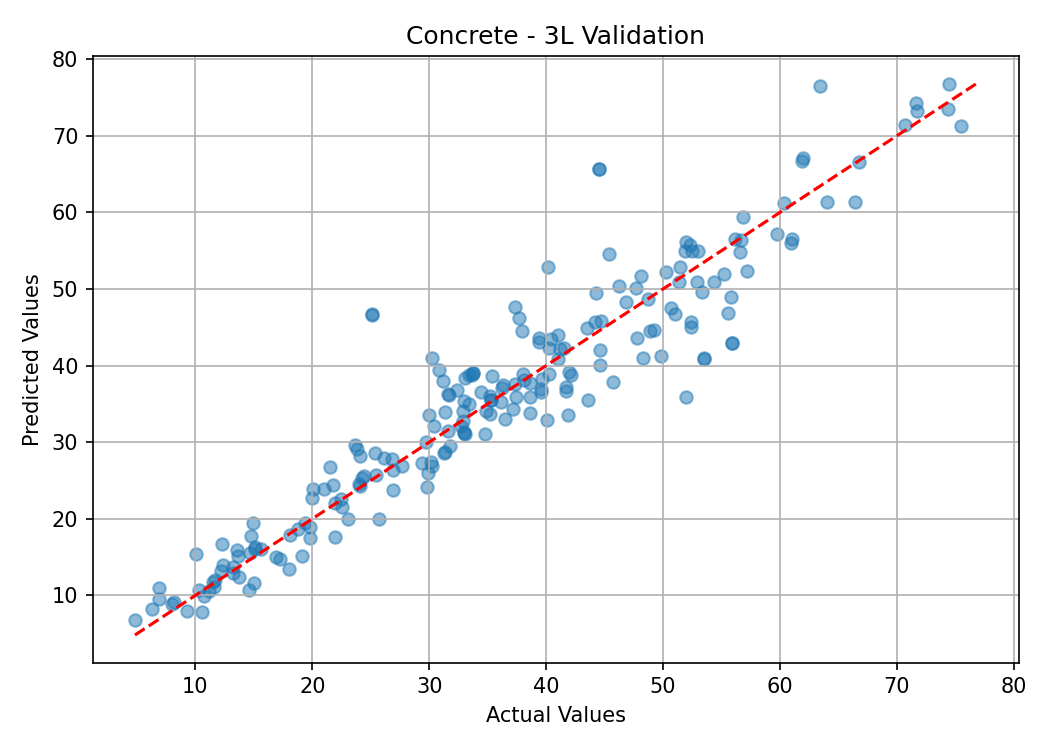
\includegraphics[width=\linewidth]{3L/pytorch_concrete_actual.png}
        \small (c) Concrete
    \end{minipage}

    \caption{PyTorch 3L Neural Network Validation Actual vs. Predicted Values}
    \label{fig:pytorch3l_actual}
\end{figure}

Figure \ref{fig:pytorch3l_actual} shows the validation actual versus predicted values, where the red dashed diagonal line represents perfect predictions. All three datasets show points clustered around the diagonal, indicating that the models capture the main trends in the data. Auto MPG follows the line closely, including the observation with the largest actual value (about 44 mpg). Airfoil and Concrete show more scatter around the line, and Concrete has a few observations with large errors, which agrees with its higher validation MSE.
\medskip
\begin{figure}[H]
    \centering

    \begin{minipage}{0.32\textwidth}
        \centering
        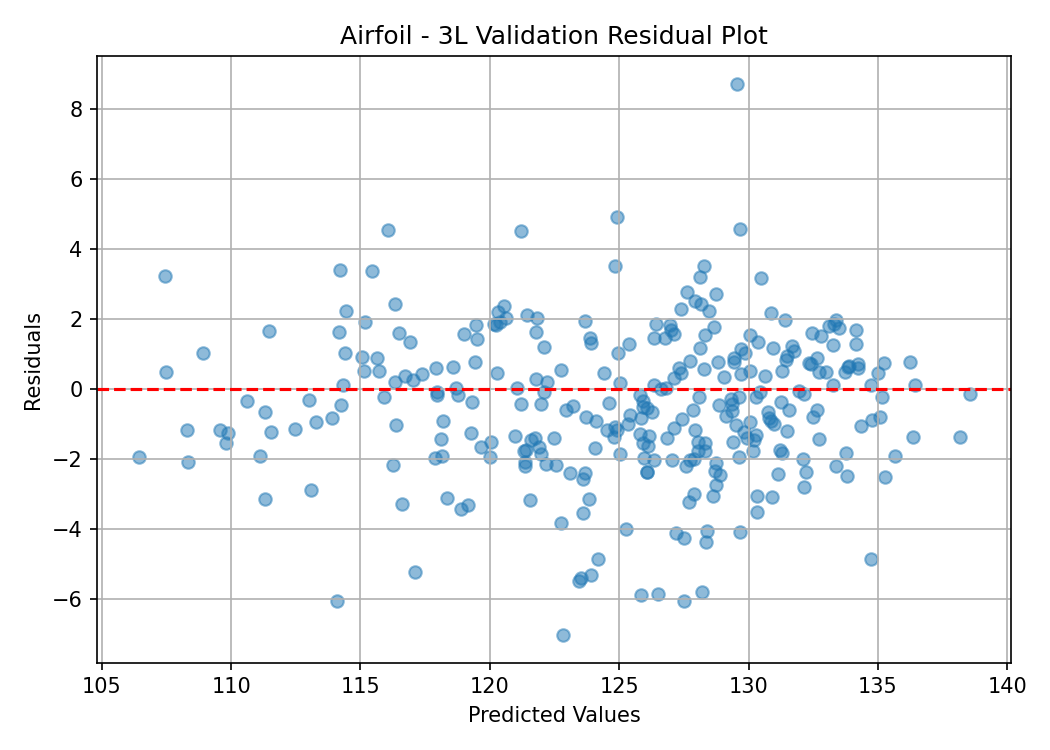
\includegraphics[width=\linewidth]{3L/pytorch_airfoil_residual.png}
        \small (a) Airfoil
    \end{minipage}
    \hfill
    \begin{minipage}{0.32\textwidth}
        \centering
        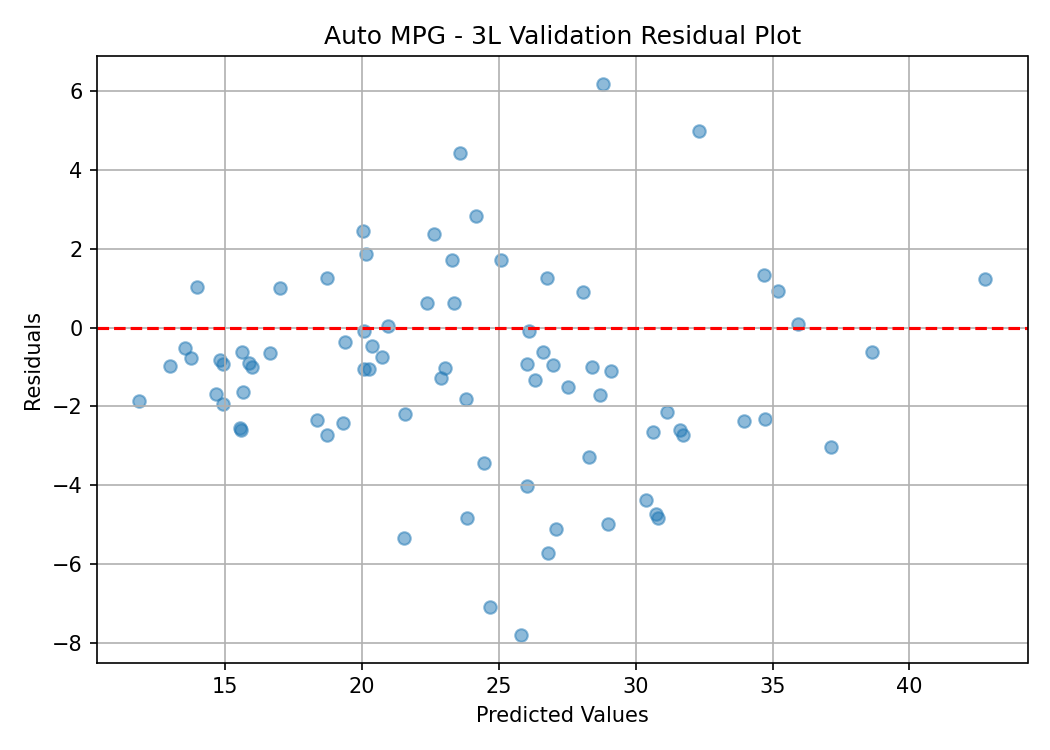
\includegraphics[width=\linewidth]{3L/pytorch_autompg_residual.png}
        \small (b) Auto MPG
    \end{minipage}
    \hfill
    \begin{minipage}{0.32\textwidth}
        \centering
        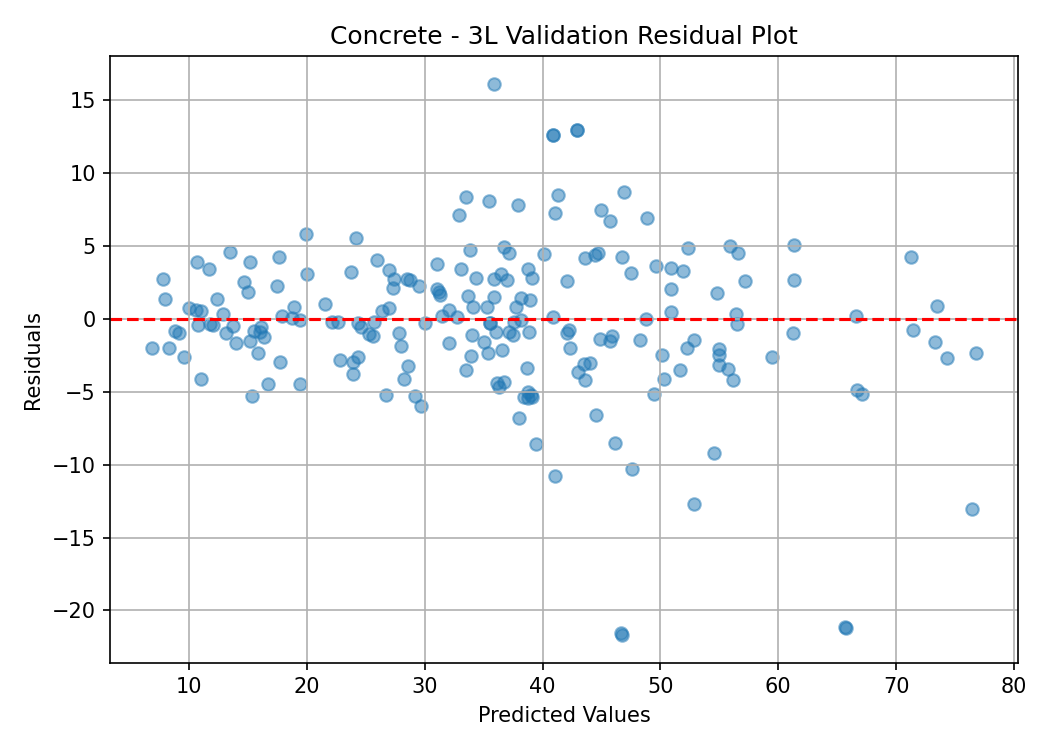
\includegraphics[width=\linewidth]{3L/pytorch_concrete_residual.png}
        \small (c) Concrete
    \end{minipage}

    \caption{PyTorch 3L Neural Network Validation Residual Plots}
    \label{fig:pytorch3l_residual}
\end{figure}

Figure \ref{fig:pytorch3l_residual} shows the validation residuals (actual minus predicted) against the predicted values, with the red dashed line marking zero error. Points above the line are underpredictions and points below are overpredictions. The Airfoil residuals are spread fairly evenly around zero with no strong pattern, mostly within $\pm$4 dB, although a few observations have errors of 6 to 9 dB. The Auto MPG residuals stay within about $\pm$8 mpg, with more points below zero for predictions between roughly 20 and 30 mpg, suggesting some overprediction in that range. The Concrete residuals have the widest spread, mostly within $\pm$10 MPa but with a few errors near $-$22 MPa. Overall, the residual plots suggest that the model captures the general relationships but still leaves noticeable error on some observations.

\subsection{Comparison and Summary}
\begin{table}[H]
    \centering
    \caption{3L Neural Network Validation $R^2$: ScalaTion vs. PyTorch, and PyTorch 2L vs. 3L}
    \label{tab:3l_comparison}
    \begin{tabular}{lccc}
        \hline
        \textbf{Dataset} & \textbf{PyTorch 2L} & \textbf{PyTorch 3L} & \textbf{ScalaTion 3L} \\
        \hline
        Airfoil  & 0.5528 & 0.9072 & 0.9287 \\
        Auto MPG & 0.7829 & 0.8526 & 0.8479 \\
        Concrete & 0.6236 & 0.8923 & 0.8986 \\
        \hline
    \end{tabular}
\end{table}

Adding a hidden layer substantially improved the PyTorch results compared with the 2L network (Table \ref{tab:3l_comparison}). Validation R² increased from 0.5528 to 0.9072 for Airfoil, from 0.7829 to 0.8526 for Auto MPG, and from 0.6236 to 0.8923 for Concrete. The largest gains were on Airfoil and Concrete, which were the two datasets where the linear 2L model performed worst, so a nonlinear hidden layer appears to help most where the relationships are more complex. Compared with the ScalaTion 3L results, PyTorch had a slightly higher validation R² on Auto MPG (0.8526 versus 0.8479), while ScalaTion was higher on Airfoil (0.9287 versus 0.9072) and slightly higher on Concrete (0.8986 versus 0.8923). The two implementations did not use identical settings: the PyTorch search was larger (180 configurations, including ReLU, 4 hidden nodes, smaller learning rates, and a batch size of 16) and used Adam with early stopping and a standardized target, while the ScalaTion search used 36 configurations trained for 400 epochs. The two implementations also used different random 80/20 splits, so their validation sets contain different observations. These differences may contribute to the differences in performance, so these comparisons should be interpreted with caution.
\medskip

Overall, the 3L neural network produced strong regression results on all three datasets in both implementations, with validation R² values between 0.85 and 0.93. In PyTorch, Airfoil showed the closest agreement between training and validation performance, while Concrete showed the largest generalization gap.


\section{4L Neural Network}
A \textbf{4-Layer Neural Network (4L)} extends the 2L architecture by adding two hidden layers between the input and output layers (input $\rightarrow$ hidden 1 $\rightarrow$ hidden 2 $\rightarrow$ output). Each hidden layer applies a linear transformation followed by a nonlinear activation function, which allows the network to learn nonlinear relationships and interactions between the predictor variables. The output layer uses the identity activation, as is standard for regression.
\medskip

For this project, the 4L Neural Network is implemented using \textbf{PyTorch} to perform regression on the same three datasets: Airfoil Self-Noise, Auto MPG, and Concrete Compressive Strength. The goal is to evaluate its predictive performance through hyperparameter tuning and Quality of Fit (QoF) measures, including R², MSE, and RMSE, for both in-sample and validation data, and to compare it with the PyTorch 2L Neural Network.

\subsection{PyTorch}
Each dataset was split into 80\% training and 20\% validation data using the same random seed as the PyTorch 2L model, so both models are evaluated on identical observations. The predictors were standardized using training data statistics. Unlike the 2L model, the target variable was also standardized using the training mean and standard deviation, since networks with hidden layers train poorly when the target is on a large raw scale (e.g., about 125 dB for Airfoil). All predictions were converted back to the original scale before calculating the QoF measures, so the MSE and RMSE values are directly comparable with the 2L results.
\medskip

Hyperparameter tuning was performed with a grid search over the number of nodes in the two hidden layers $\{(16, 8), (32, 16), (64, 32), (128, 64)\}$, the activation function $\{$ReLU, Tanh, Sigmoid$\}$, the mini-batch size $\{16, 32, 64\}$, and the learning rate $\{0.001, 0.005, 0.01, 0.05\}$, giving 144 configurations per dataset. Each configuration was trained with the Adam optimizer for a maximum of 300 epochs with early stopping (patience = 20), using an inner 80/20 split of the training data, so the 20\% validation set was never used during tuning. The final model for each dataset was then retrained on the full training set for the best number of epochs found during tuning.
\medskip
\begin{table}[H]
    \centering
    \caption{PyTorch 4L Neural Network Hyperparameter Tuning Results}
    \label{tab:pytorch4l_hyperparameters}
    \small
    \begin{tabular}{lcccccc}
        \hline
        \textbf{Dataset} & \textbf{Hidden Nodes} & \textbf{Activation} & \textbf{Learning Rate} & \textbf{Batch Size} & \textbf{Validation MSE} & \textbf{Best Epoch} \\
        \hline
        Airfoil  & (128, 64) & ReLU & 0.001 & 16 & 3.0190 & 225 \\
        Auto MPG & (64, 32) & Tanh & 0.050 & 32 & 5.9313 & 14 \\
        Concrete & (64, 32) & ReLU & 0.005 & 64 & 15.8281 & 86 \\
        \hline
    \end{tabular}
\end{table}

As shown in Table \ref{tab:pytorch4l_hyperparameters}, the selected hyperparameters differ across datasets. ReLU was selected for Airfoil and Concrete, while Tanh was selected for Auto MPG. Airfoil selected the largest network (128 and 64 nodes) with the smallest learning rate (0.001), which required 225 epochs to reach its best validation loss. Since this configuration lies on the edge of the search space, a larger network or smaller learning rate may improve Airfoil further. Auto MPG reached its best validation loss after only 14 epochs with a high learning rate of 0.05, which reflects its small size (250 tuning observations). The tuning validation MSE values are much lower than those of the 2L model (Table \ref{tab:pytorch_hyperparameters}), e.g., 3.02 vs. 31.51 for Airfoil and 15.83 vs. 106.18 for Concrete.
\medskip
\begin{figure}[H]
    \centering
    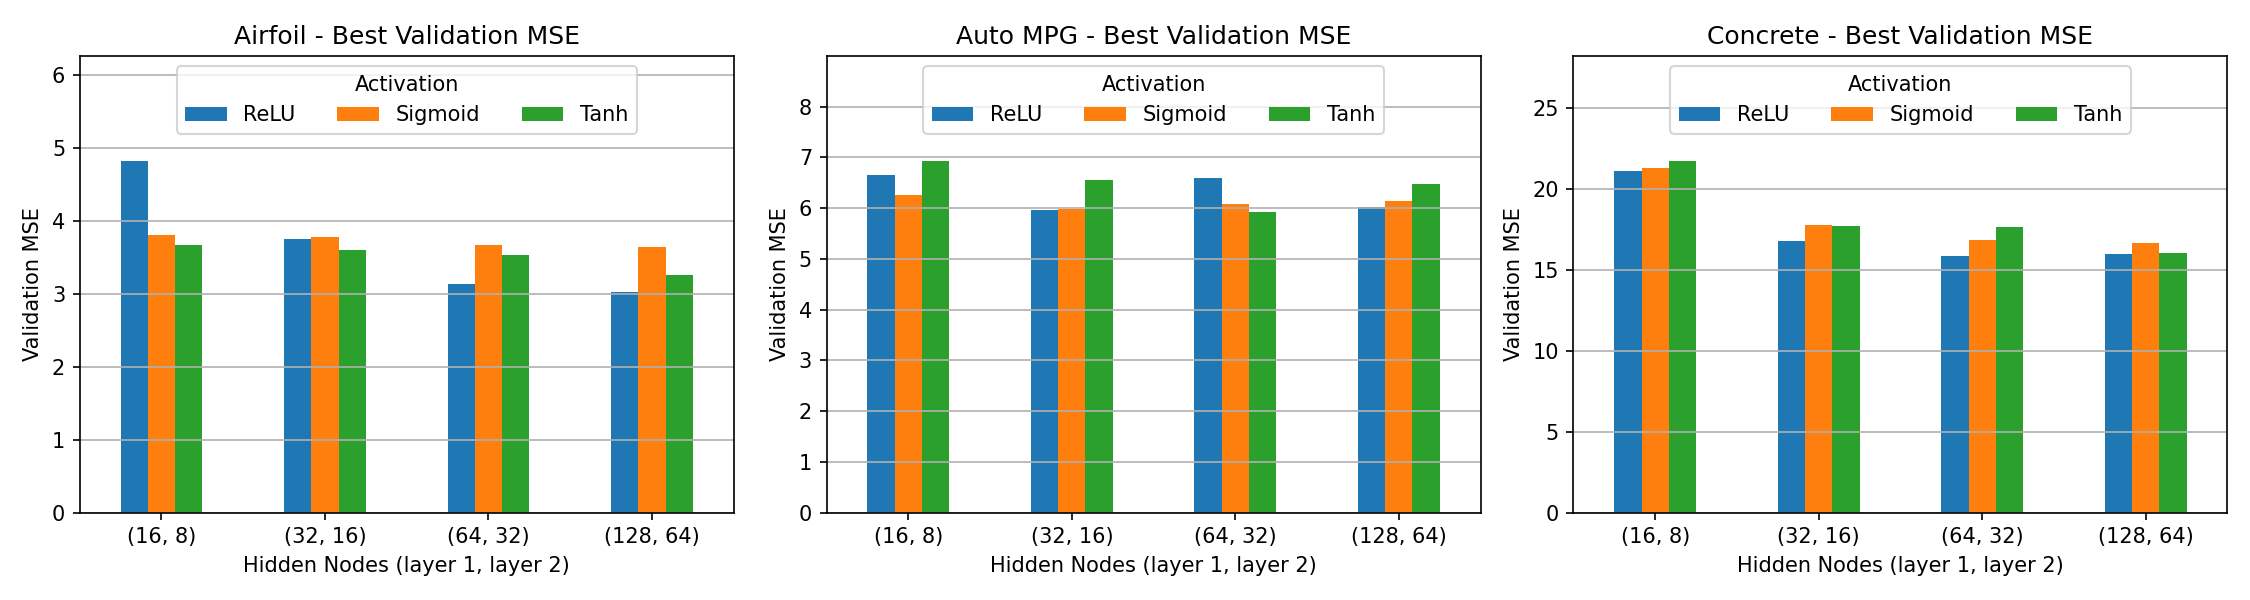
\includegraphics[width=\linewidth]{4L/tuning_sensitivity.png}
    \caption{PyTorch 4L Best Tuning Validation MSE by Hidden Layer Size and Activation Function}
    \label{fig:pytorch4l_tuning}
\end{figure}

Figure \ref{fig:pytorch4l_tuning} shows the best tuning validation MSE for each hidden layer size and activation function. For Airfoil and Concrete, the validation MSE generally decreases as the number of hidden nodes increases: the smallest network (16, 8) performs worst on both datasets, and ReLU performs best for the larger networks. For Concrete, the largest improvement occurs between (16, 8) and (32, 16), while Airfoil continues to improve up to (128, 64). For Auto MPG, the differences across sizes and activation functions are small (about 5.9 to 6.9), suggesting that its relationships are simple enough that network size has little effect.
\medskip
\begin{table}[H]
    \centering
    \caption{PyTorch 4L Neural Network Quality of Fit Results}
    \label{tab:pytorch4l_qof}
    \small
    \resizebox{\textwidth}{!}{
    \begin{tabular}{lcccccc}
        \hline
        \textbf{Dataset} & \textbf{Train $R^2$} & \textbf{Validation $R^2$} & \textbf{Train MSE} & \textbf{Validation MSE} & \textbf{Train RMSE} & \textbf{Validation RMSE} \\
        \hline
        Airfoil  & 0.9720 & 0.9643 & 1.3152 & 1.7895 & 1.1468 & 1.3377 \\
        Auto MPG & 0.8581 & 0.8317 & 8.9528 & 8.5903 & 2.9921 & 2.9309 \\
        Concrete & 0.9623 & 0.8691 & 10.6965 & 33.7271 & 3.2706 & 5.8075 \\
        \hline
    \end{tabular}
    }
\end{table}

The Quality of Fit (QoF) results were evaluated using R², MSE, and RMSE for both in-sample (training) and validation data. As shown in Table \ref{tab:pytorch4l_qof}, Airfoil achieved the highest validation R² of 0.9643, followed by Concrete at 0.8691 and Auto MPG at 0.8317. Airfoil's training and validation R² values are very close, indicating that the model generalizes well. Concrete shows the largest gap between training (0.9623) and validation (0.8691) R², and its validation MSE (33.73) is about three times its training MSE (10.70), indicating some overfitting. Auto MPG shows a small gap, and its validation MSE is slightly lower than its training MSE, which can occur with a small validation set of 79 observations. To check that these results do not depend on a single random initialization, the final models were retrained with five different seeds. The mean validation R² values were 0.9610 ($\pm$0.0082) for Airfoil, 0.8525 ($\pm$0.0255) for Auto MPG, and 0.8738 ($\pm$0.0111) for Concrete, consistent with Table \ref{tab:pytorch4l_qof}.
\medskip
\begin{figure}[H]
    \centering

    \begin{minipage}{0.32\textwidth}
        \centering
        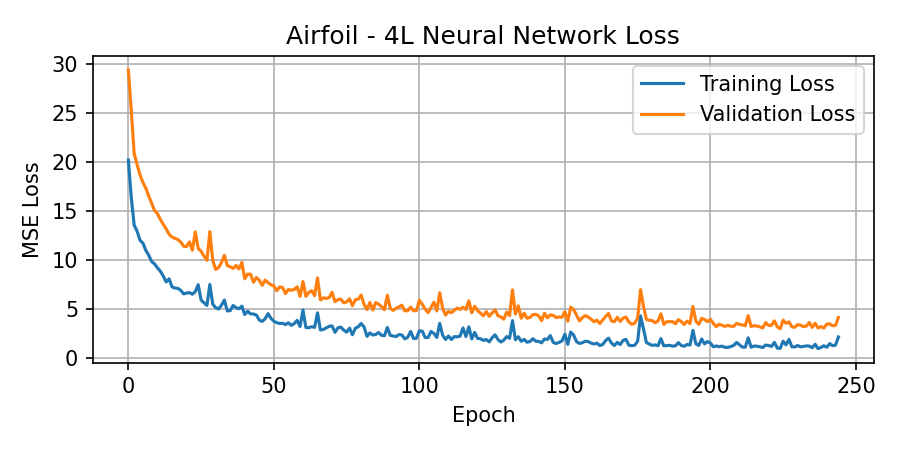
\includegraphics[width=\linewidth]{4L/airfoil_loss.png}
        \small (a) Airfoil
    \end{minipage}
    \hfill
    \begin{minipage}{0.32\textwidth}
        \centering
        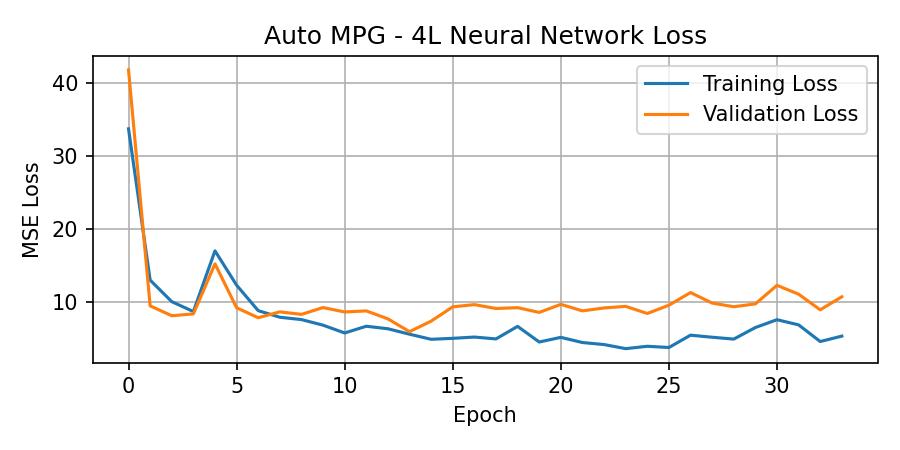
\includegraphics[width=\linewidth]{4L/autompg_loss.png}
        \small (b) Auto MPG
    \end{minipage}
    \hfill
    \begin{minipage}{0.32\textwidth}
        \centering
        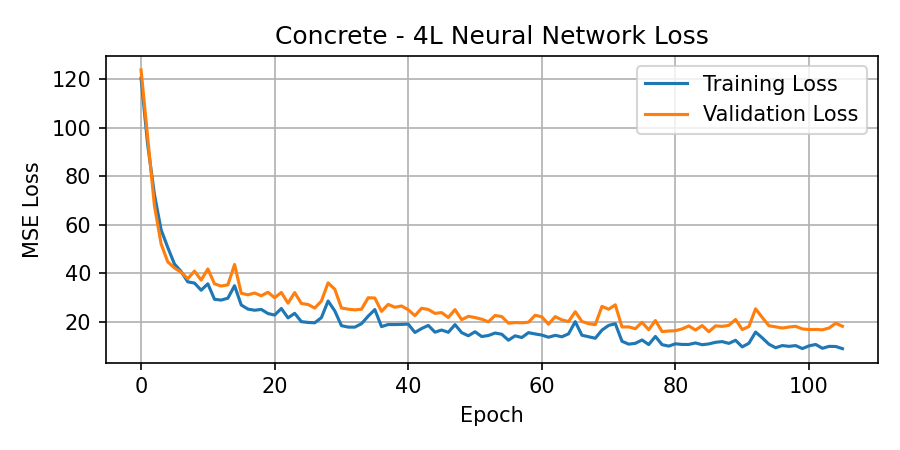
\includegraphics[width=\linewidth]{4L/concrete_loss.png}
        \small (c) Concrete
    \end{minipage}

    \caption{PyTorch 4L Neural Network Training and Validation Loss vs. Epoch}
    \label{fig:pytorch4l_loss}
\end{figure}

Figure \ref{fig:pytorch4l_loss} shows the training and validation loss vs epoch plots for the best configuration of each dataset. Airfoil shows a steady decrease in both losses over about 225 epochs, with the validation loss remaining close to the training loss. Auto MPG drops sharply within the first few epochs and reaches its best validation loss at epoch 14; after that, the training loss keeps decreasing while the validation loss slowly rises, which is an early sign of overfitting that early stopping prevents. Concrete decreases steadily, but the gap between the training and validation losses widens after roughly 70 epochs, consistent with its larger training--validation gap in Table \ref{tab:pytorch4l_qof}. Compared with the 2L loss curves (Figure \ref{fig:pytorch_loss}), the 4L curves are noisier, which is expected from the larger number of parameters and the use of mini-batches.
\medskip
\begin{figure}[H]
    \centering

    \begin{minipage}{0.32\textwidth}
        \centering
        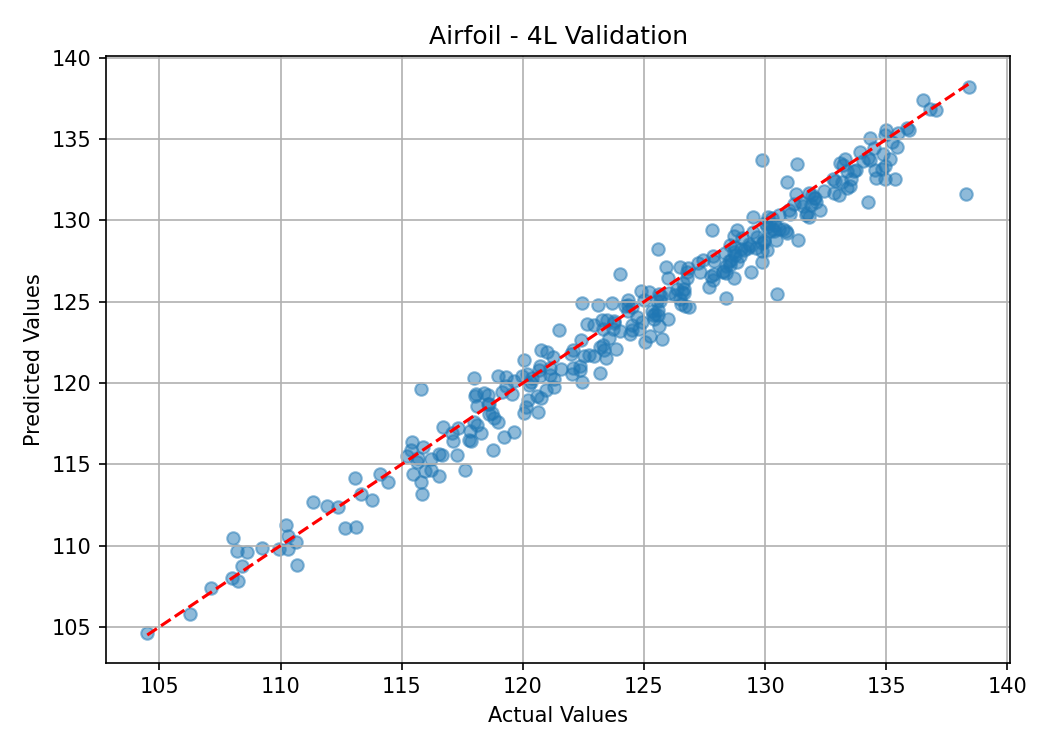
\includegraphics[width=\linewidth]{4L/airfoil_actual.png}
        \small (a) Airfoil
    \end{minipage}
    \hfill
    \begin{minipage}{0.32\textwidth}
        \centering
        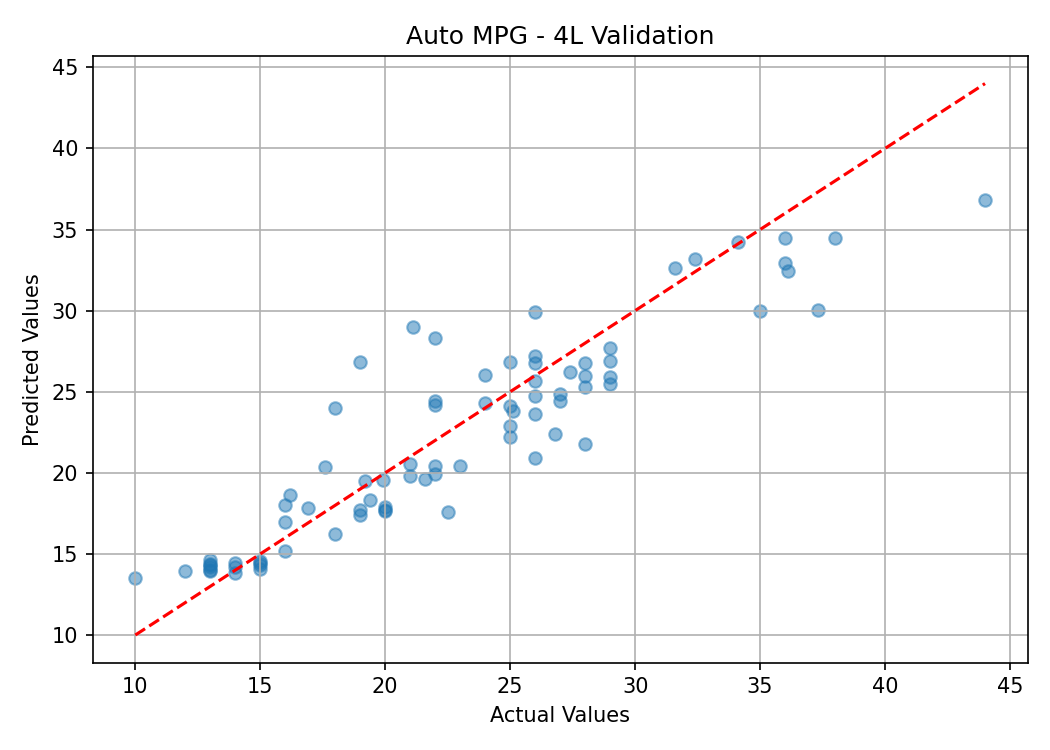
\includegraphics[width=\linewidth]{4L/autompg_actual.png}
        \small (b) Auto MPG
    \end{minipage}
    \hfill
    \begin{minipage}{0.32\textwidth}
        \centering
        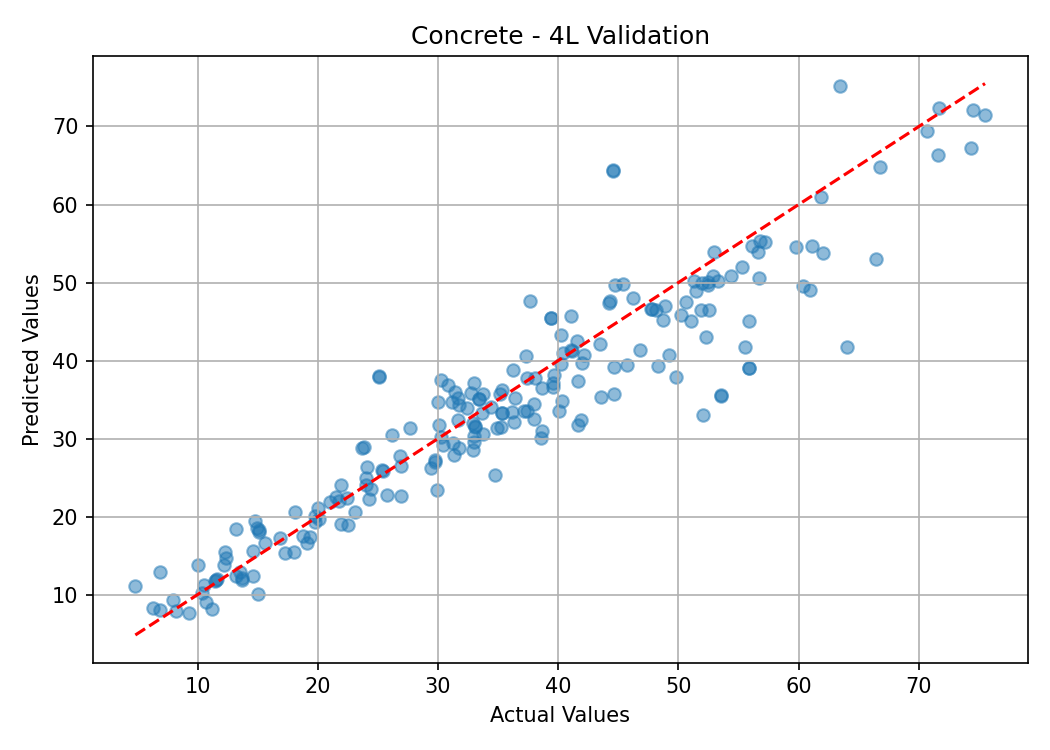
\includegraphics[width=\linewidth]{4L/concrete_actual.png}
        \small (c) Concrete
    \end{minipage}

    \caption{PyTorch 4L Neural Network Validation Actual vs. Predicted Values}
    \label{fig:pytorch4l_actual}
\end{figure}

Figure \ref{fig:pytorch4l_actual} shows the validation actual vs predicted plots for the three datasets. The red dashed diagonal line represents perfect predictions. Airfoil's points lie tightly along the diagonal line across the full range of sound pressure levels, a large improvement over the 2L model (Figure \ref{fig:pytorch_actual}). Concrete also follows the diagonal closely, with more spread at mid-range strengths (30--55 MPa). Auto MPG follows the diagonal for most observations but underestimates the highest-mpg cars (e.g., an actual value of 44 mpg is predicted at about 37 mpg).
\medskip
\begin{figure}[H]
    \centering

    \begin{minipage}{0.32\textwidth}
        \centering
        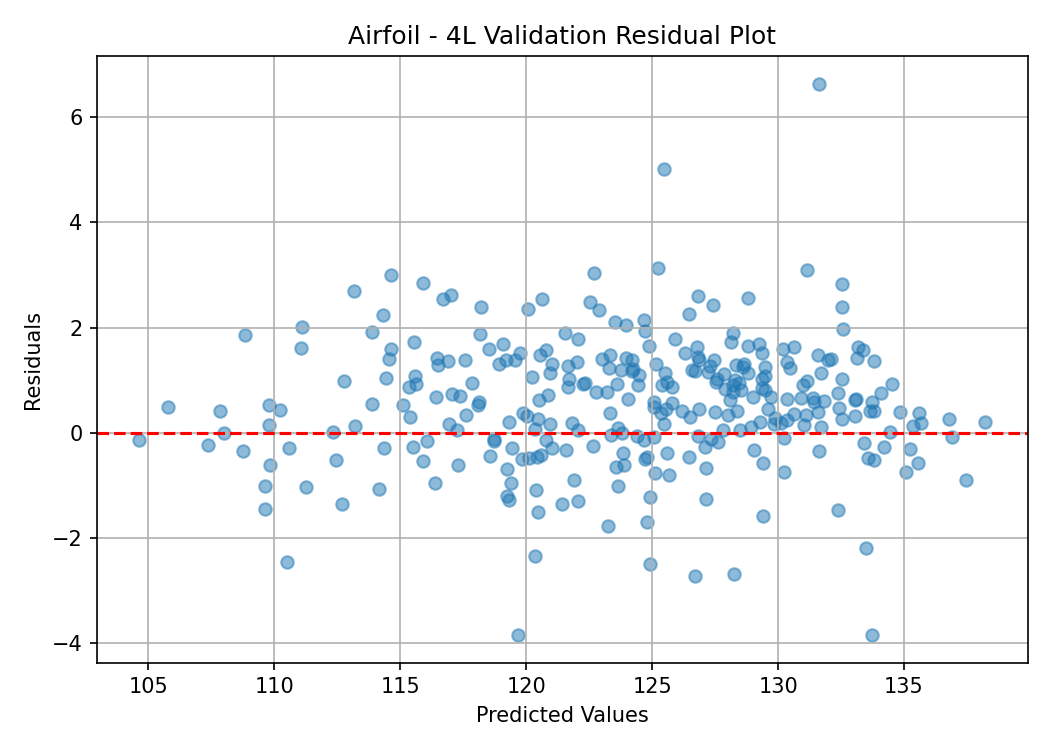
\includegraphics[width=\linewidth]{4L/airfoil_residual.png}
        \small (a) Airfoil
    \end{minipage}
    \hfill
    \begin{minipage}{0.32\textwidth}
        \centering
        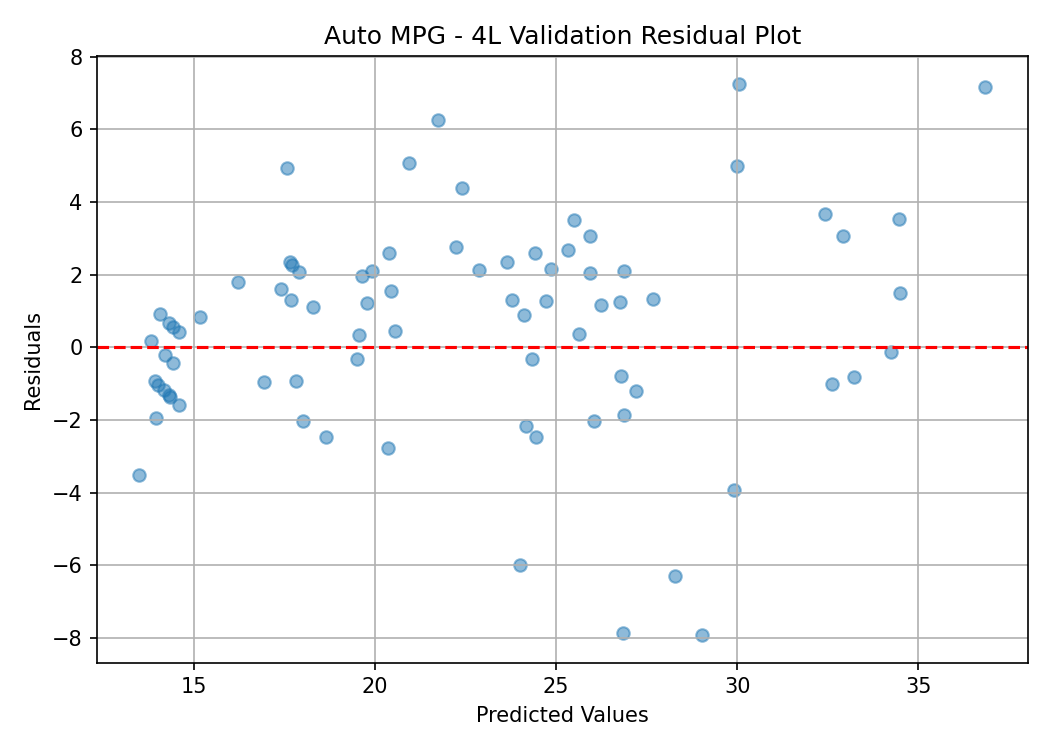
\includegraphics[width=\linewidth]{4L/autompg_residual.png}
        \small (b) Auto MPG
    \end{minipage}
    \hfill
    \begin{minipage}{0.32\textwidth}
        \centering
        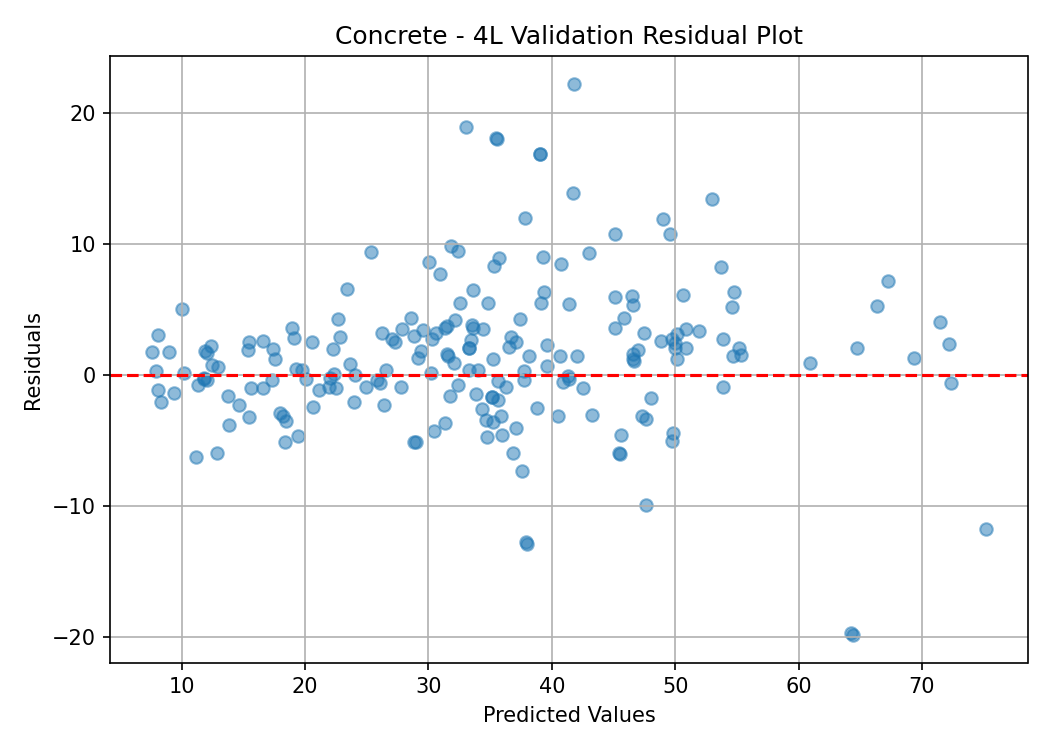
\includegraphics[width=\linewidth]{4L/concrete_residual.png}
        \small (c) Concrete
    \end{minipage}

    \caption{PyTorch 4L Neural Network Validation Residual Plots}
    \label{fig:pytorch4l_residual}
\end{figure}

Figure \ref{fig:pytorch4l_residual} shows the validation residual plots for the three datasets. Airfoil's residuals are small (mostly within $\pm$3 dB) and show no clear pattern, indicating that the hidden layers capture the nonlinear structure that the 2L model missed (its validation RMSE drops from 4.73 to 1.34 dB). However, about 71\% of the Airfoil residuals are positive, indicating that the model slightly underestimates sound pressure on the validation set. Auto MPG's residuals are mostly within $\pm$4 mpg, and the curved pattern seen in the 2L residuals (Figure \ref{fig:pytorch_residual}) is no longer present. Concrete's residuals are centered around zero but spread more widely at mid-range predicted values, with a few large errors near $\pm$20 MPa. All three models have a small positive mean validation residual (0.56 dB, 0.55 mpg, and 1.43 MPa), so they tend to slightly underpredict on unseen data. The Concrete dataset also contains 34 rows with duplicated predictor values, so a small number of validation rows have an identical input in the training set; this affects the 2L and 4L models equally.

\subsection{Comparison with the 2L Neural Network}
\begin{table}[H]
    \centering
    \caption{PyTorch 2L vs. 4L Neural Network Validation $R^2$}
    \label{tab:pytorch_2l_vs_4l}
    \begin{tabular}{lccc}
        \hline
        \textbf{Dataset} & \textbf{2L Validation $R^2$} & \textbf{4L Validation $R^2$} & \textbf{Improvement} \\
        \hline
        Airfoil  & 0.5528 & 0.9643 & +0.4115 \\
        Auto MPG & 0.7829 & 0.8317 & +0.0488 \\
        Concrete & 0.6236 & 0.8691 & +0.2455 \\
        \hline
    \end{tabular}
\end{table}

Table \ref{tab:pytorch_2l_vs_4l} compares the validation R² of the PyTorch 2L and 4L models, which use identical training and validation splits. The 4L model improved validation R² on all three datasets. The largest improvement was for Airfoil (+0.41), whose relationship between frequency, boundary layer thickness, and sound pressure is strongly nonlinear and cannot be captured by the 2L model's linear prediction. Concrete also improved substantially (+0.25), as compressive strength depends nonlinearly on ingredient ratios and curing age. Auto MPG improved the least (+0.05), since a linear model already explains most of its variation. These results also change the ranking of the datasets: Auto MPG had the highest validation R² with the 2L model, but it has the lowest with the 4L model.

\subsection{Conclusion}
Overall, adding two hidden layers greatly improved predictive performance compared with the 2L Neural Network, raising validation R² from 0.55 to 0.96 for Airfoil and from 0.62 to 0.87 for Concrete. The improvement depends on how nonlinear each dataset is: Airfoil and Concrete benefited the most, while Auto MPG, which is close to linear, improved only slightly. The added flexibility also increased the risk of overfitting, most visibly for Concrete, where the training R² (0.96) exceeds the validation R² (0.87). Hyperparameter tuning showed that the best settings vary by dataset, with ReLU and larger hidden layers working best for the two larger datasets. Early stopping was important for controlling overfitting, especially for the small Auto MPG dataset.

\section{5L Neural Network}
A \textbf{5-Layer Neural Network (5L)} has an input layer, three hidden layers, and an output layer. Each hidden layer applies a linear transformation followed by a nonlinear activation function, and the output layer uses the identity activation because all three tasks predict continuous numerical responses.

\subsection{PyTorch}

\subsubsection{Methodology}
A five-layer neural network (5L) was implemented using \textbf{PyTorch} to perform regression on the Airfoil Self-Noise, Auto MPG, and Concrete Compressive Strength datasets. Each network consisted of an input layer, three hidden layers, and an output layer. The number of nodes in each hidden layer, hidden-layer activation function, learning rate, and mini-batch size were tuned to identify a configuration with low validation error. The output layer used an identity activation function because all three tasks predict continuous numerical responses.
\medskip

The Airfoil, Auto MPG, and Concrete datasets contained 1,503, 392, and 1,030 observations, respectively. Their networks used 5, 7, and 8 input features, respectively. Each dataset was divided into an outer 80/20 training-validation split using the same random seed as the PyTorch 2L and 4L models, so all three models are evaluated on identical observations. Input features were standardized using statistics calculated from the training data. As in the 4L model, the target variable was also standardized using the training mean and standard deviation, and predictions were converted back to the original scale before calculating the QoF measures. Hyperparameter selection used an additional validation split within the outer training portion, keeping the final held-out validation data separate from hyperparameter selection.
\medskip

The hyperparameter search evaluated 96 configurations per dataset. It considered four hidden-layer layouts: (8, 8, 8), (16, 16, 16), (32, 16, 8), and (64, 32, 16); ReLU and hyperbolic tangent (tanh) activation functions; learning rates of 0.001, 0.005, 0.01, and 0.05; and mini-batch sizes of 16, 32, and 64. Each configuration was trained with the Adam optimizer for a maximum of 300 epochs with early stopping (patience = 20) based on the inner-validation MSE. The configuration with the lowest inner-validation mean squared error (MSE) was selected for each dataset. The final model was then retrained on the full training set using the selected configuration for the number of epochs at which the inner-validation MSE was lowest, and evaluated on the held-out validation set.
\medskip

The ReLU activation function (Figure \ref{fig:relu}) is defined as $f(x) = \max(0, x)$. It returns zero for negative inputs and returns the input itself for nonnegative inputs.
\begin{figure}[H]
    \centering
    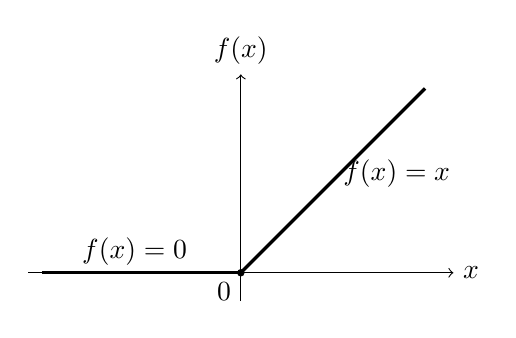
\begin{tikzpicture}[scale=0.9]
        \draw[->] (-3,0) -- (3,0) node[right] {$x$};
        \draw[->] (0,-0.4) -- (0,2.8) node[above] {$f(x)$};
        \draw[very thick] (-2.8,0) -- (0,0);
        \draw[very thick] (0,0) -- (2.6,2.6);
        \fill (0,0) circle (1.5pt);
        \node at (-1.5,0.3) {$f(x) = 0$};
        \node at (2.2,1.4) {$f(x) = x$};
        \node[below left] at (0,0) {$0$};
    \end{tikzpicture}
    \caption{ReLU Activation Function, $f(x) = \max(0, x)$}
    \label{fig:relu}
\end{figure}

\subsubsection{Hyperparameter-Tuning Results}
\begin{table}[H]
    \centering
    \caption{PyTorch 5L Neural Network Hyperparameter Tuning Results}
    \label{tab:pytorch5l_hyperparameters}
    \small
    \begin{tabular}{lcccccc}
        \hline
        \textbf{Dataset} & \textbf{Hidden Layers} & \textbf{Activation} & \textbf{Learning Rate} & \textbf{Batch Size} & \textbf{Inner-Val. MSE} & \textbf{Best Epoch} \\
        \hline
        Airfoil  & (16, 16, 16) & tanh & 0.01 & 32 & 3.1975 & 132 \\
        Auto MPG & (16, 16, 16) & ReLU & 0.05 & 16 & 5.4647 & 26 \\
        Concrete & (64, 32, 16) & ReLU & 0.01 & 32 & 15.6003 & 66 \\
        \hline
    \end{tabular}
\end{table}

As shown in Table \ref{tab:pytorch5l_hyperparameters}, the selected configurations varied across the three datasets. ReLU was selected for Auto MPG and Concrete, while tanh was selected for Airfoil. Concrete selected the widest hidden-layer layout tested, (64, 32, 16), while Airfoil and Auto MPG selected (16, 16, 16). Auto MPG selected the largest learning rate tested (0.05), so a wider learning-rate range could be explored in future work. These are the best configurations within the tested search grid; they do not establish that the configurations are globally optimal.

\subsubsection{Quality of Fit}
The final models were evaluated using the coefficient of determination (R²), MSE, and root mean squared error (RMSE). Training and held-out validation results are reported in Table \ref{tab:pytorch5l_qof}.
\begin{table}[H]
    \centering
    \caption{PyTorch 5L Neural Network Quality of Fit Results}
    \label{tab:pytorch5l_qof}
    \small
    \resizebox{\textwidth}{!}{
    \begin{tabular}{lcccccc}
        \hline
        \textbf{Dataset} & \textbf{Train $R^2$} & \textbf{Validation $R^2$} & \textbf{Train MSE} & \textbf{Validation MSE} & \textbf{Train RMSE} & \textbf{Validation RMSE} \\
        \hline
        Airfoil  & 0.9720 & 0.9618 & 1.3151 & 1.9116 & 1.1468 & 1.3826 \\
        Auto MPG & 0.8902 & 0.8813 & 6.9298 & 6.0568 & 2.6325 & 2.4611 \\
        Concrete & 0.9491 & 0.8723 & 14.4641 & 32.8990 & 3.8032 & 5.7358 \\
        \hline
    \end{tabular}
    }
\end{table}

The Airfoil model achieved the strongest validation R² at 0.9618 and close agreement between training and validation scores. Its validation RMSE was 1.3826 dB. The Auto MPG model achieved a validation R² of 0.8813, close to its training R² of 0.8902, and its validation MSE was slightly lower than its training MSE, which can occur with a small validation set of 79 observations. The Concrete model achieved a validation R² of 0.8723 and a validation RMSE of 5.7358 MPa. Its validation MSE (32.90) is more than twice its training MSE (14.46), giving the largest training--validation gap of the three datasets and indicating some overfitting.
\medskip

To check how much these results depend on the random initialization, the final models were retrained with five different seeds (Table \ref{tab:pytorch5l_seeds}). Airfoil and Concrete are stable, but the Auto MPG validation R² ranges from 0.7540 to 0.8758 depending on the seed. Its single-seed result in Table \ref{tab:pytorch5l_qof} is therefore on the high end, and the five-seed mean of 0.8269 is a more reliable estimate. This instability is likely caused by the combination of a small dataset and the high learning rate of 0.05, which also makes its loss curve noisy (Figure \ref{fig:pytorch5l_loss}).
\begin{table}[H]
    \centering
    \caption{PyTorch 5L Validation $R^2$ over Five Random Seeds}
    \label{tab:pytorch5l_seeds}
    \small
    \begin{tabular}{lcccc}
        \hline
        \textbf{Dataset} & \textbf{Mean} & \textbf{Std. Dev.} & \textbf{Min} & \textbf{Max} \\
        \hline
        Airfoil  & 0.9506 & 0.0074 & 0.9365 & 0.9558 \\
        Auto MPG & 0.8269 & 0.0472 & 0.7540 & 0.8758 \\
        Concrete & 0.8795 & 0.0122 & 0.8690 & 0.8961 \\
        \hline
    \end{tabular}
\end{table}

\subsubsection{Loss, Prediction, and Residual Plots}
\begin{figure}[H]
    \centering

    \begin{minipage}{0.32\textwidth}
        \centering
        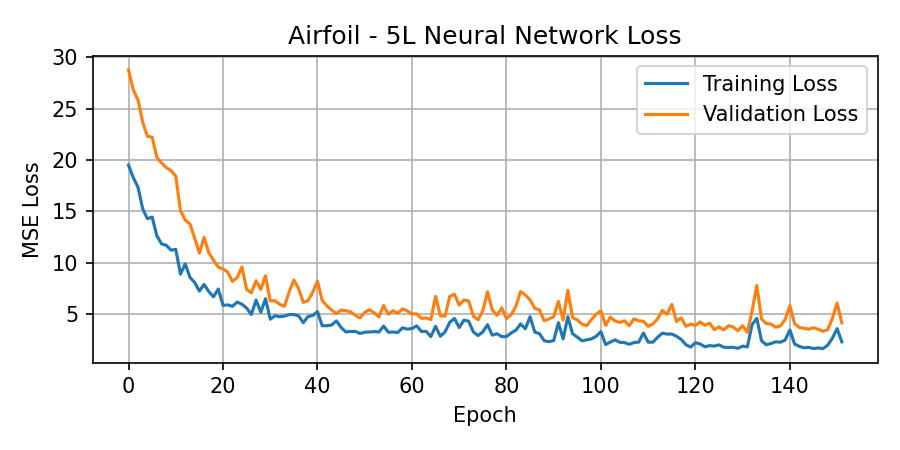
\includegraphics[width=\linewidth]{5L/airfoil_loss.png}
        \small (a) Airfoil
    \end{minipage}
    \hfill
    \begin{minipage}{0.32\textwidth}
        \centering
        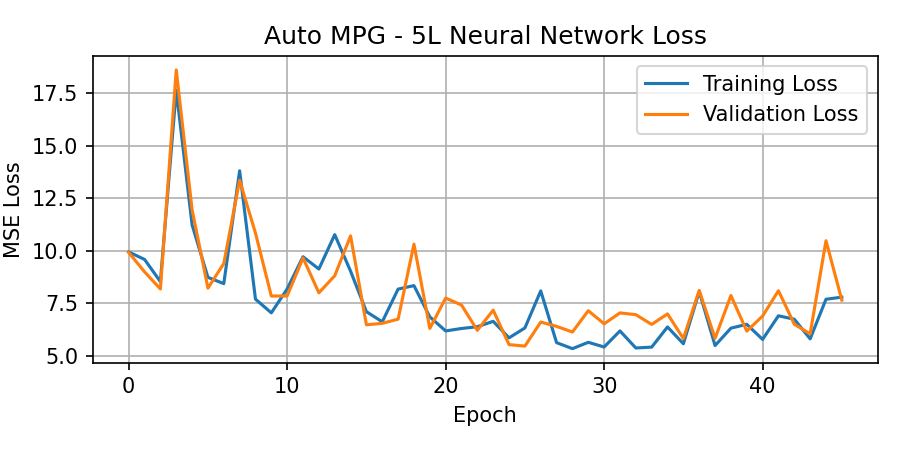
\includegraphics[width=\linewidth]{5L/autompg_loss.png}
        \small (b) Auto MPG
    \end{minipage}
    \hfill
    \begin{minipage}{0.32\textwidth}
        \centering
        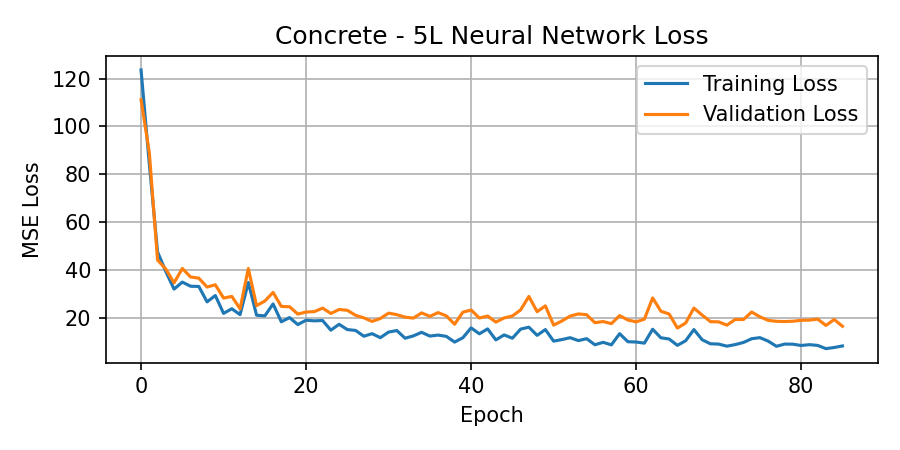
\includegraphics[width=\linewidth]{5L/concrete_loss.png}
        \small (c) Concrete
    \end{minipage}

    \caption{PyTorch 5L Neural Network Training and Validation Loss vs. Epoch (Tuning Run, Selected Configuration)}
    \label{fig:pytorch5l_loss}
\end{figure}

Figure \ref{fig:pytorch5l_loss} shows the training and inner-validation loss for the selected configuration of each dataset. Airfoil decreases steadily until about epoch 130, with the validation loss staying slightly above the training loss. Concrete drops sharply in the first few epochs, after which a gap between the training and validation losses opens, consistent with its larger training--validation gap in Table \ref{tab:pytorch5l_qof}. Auto MPG is the noisiest, with a large spike near epoch 3 and continued fluctuations, reflecting its high learning rate and small number of observations.
\medskip
\begin{figure}[H]
    \centering
    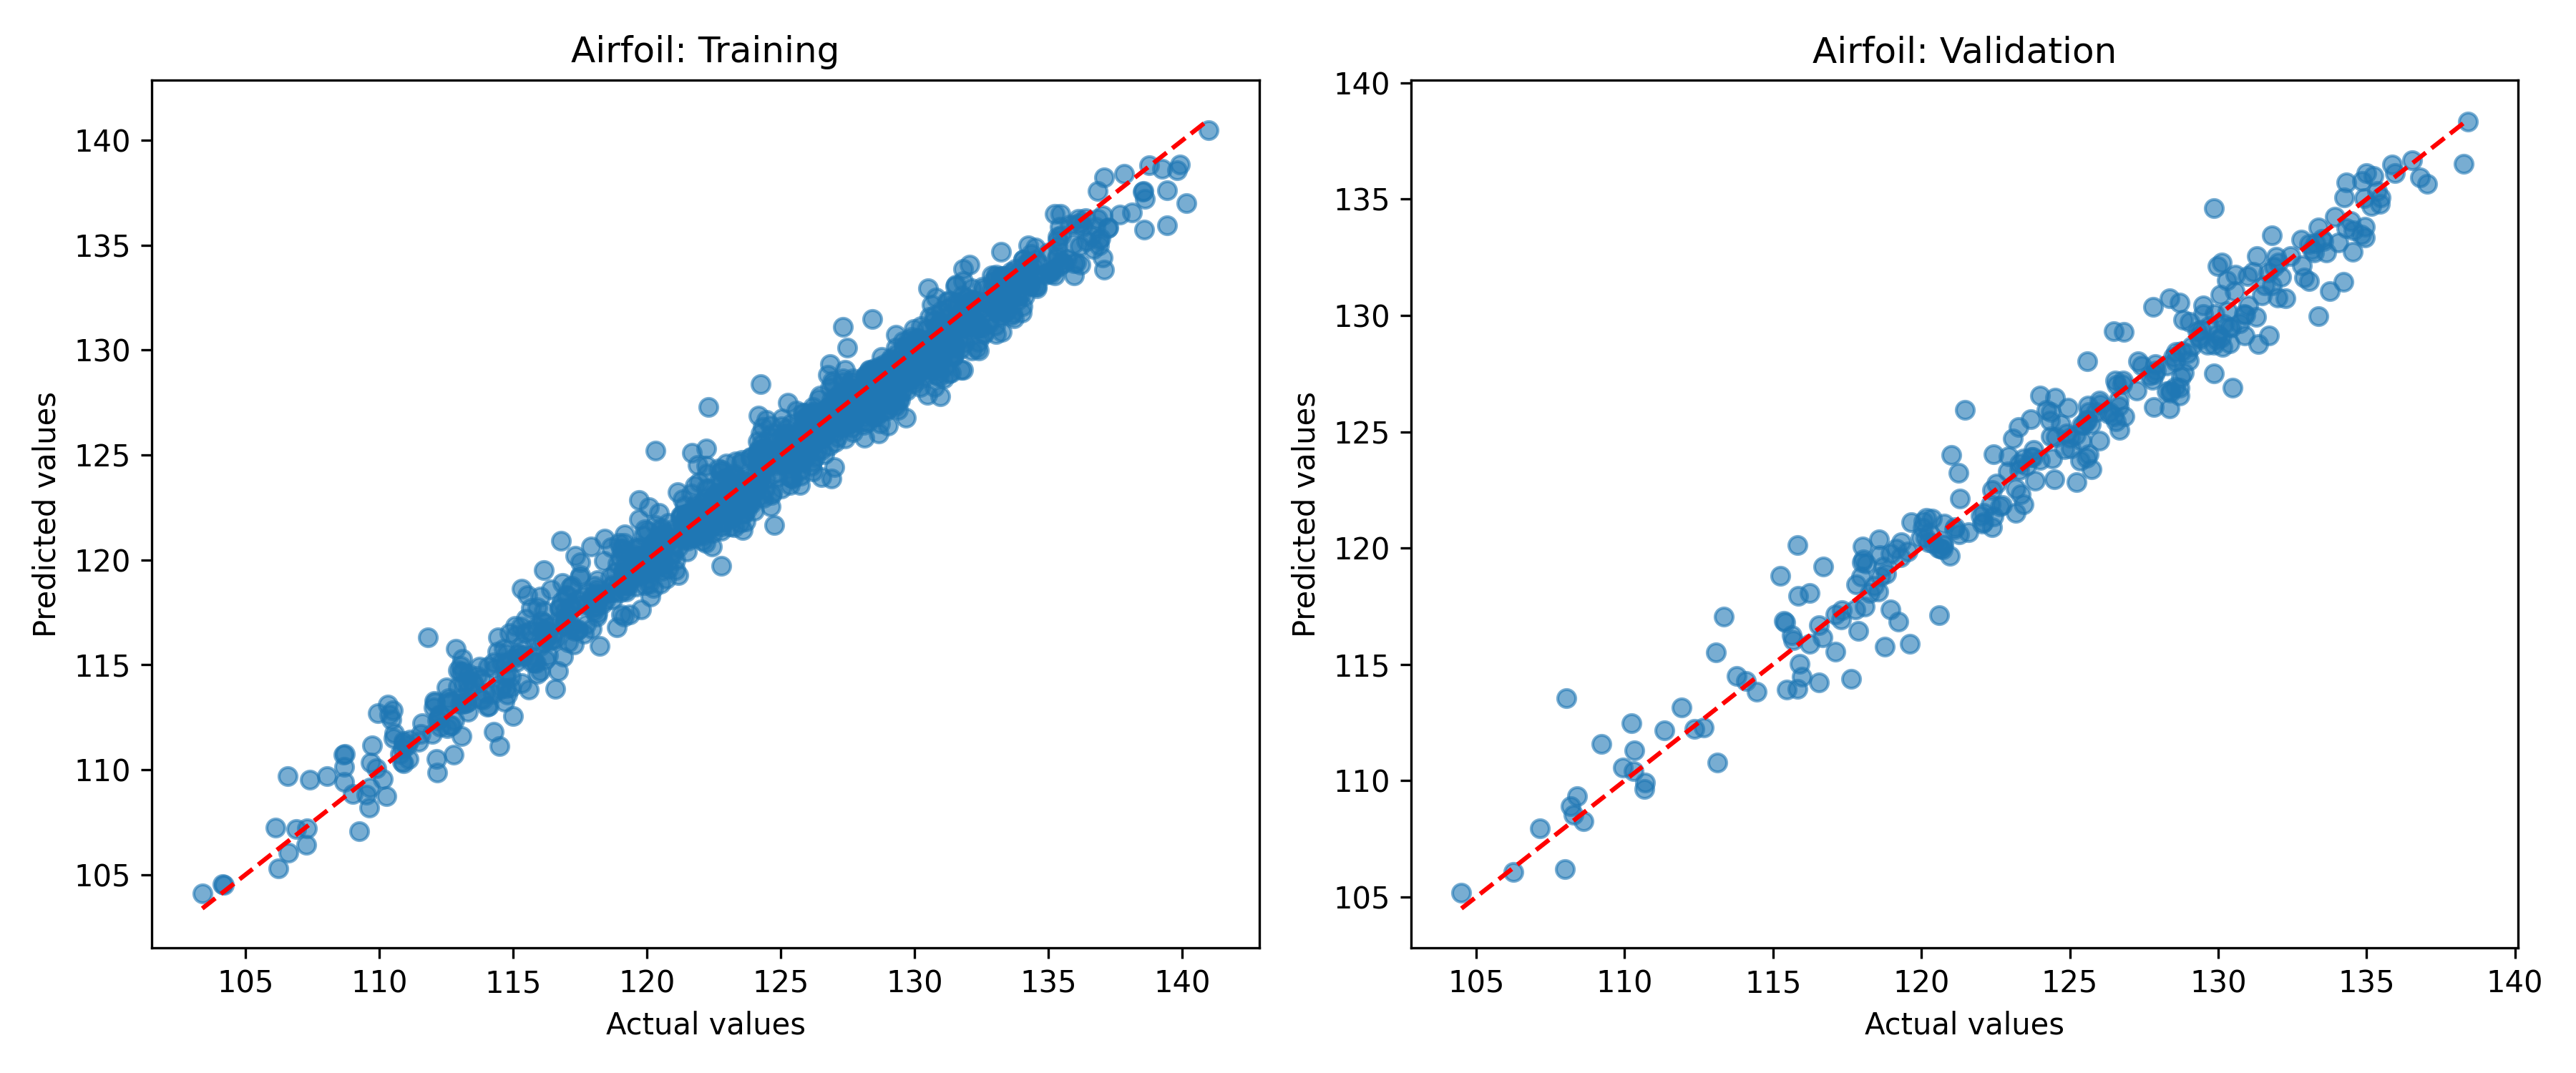
\includegraphics[width=0.85\linewidth]{5L/airfoil_actual.png}
    \caption{PyTorch 5L Actual vs. Predicted Values for Airfoil (Left: Training, Right: Validation)}
    \label{fig:pytorch5l_airfoil}
\end{figure}
\begin{figure}[H]
    \centering
    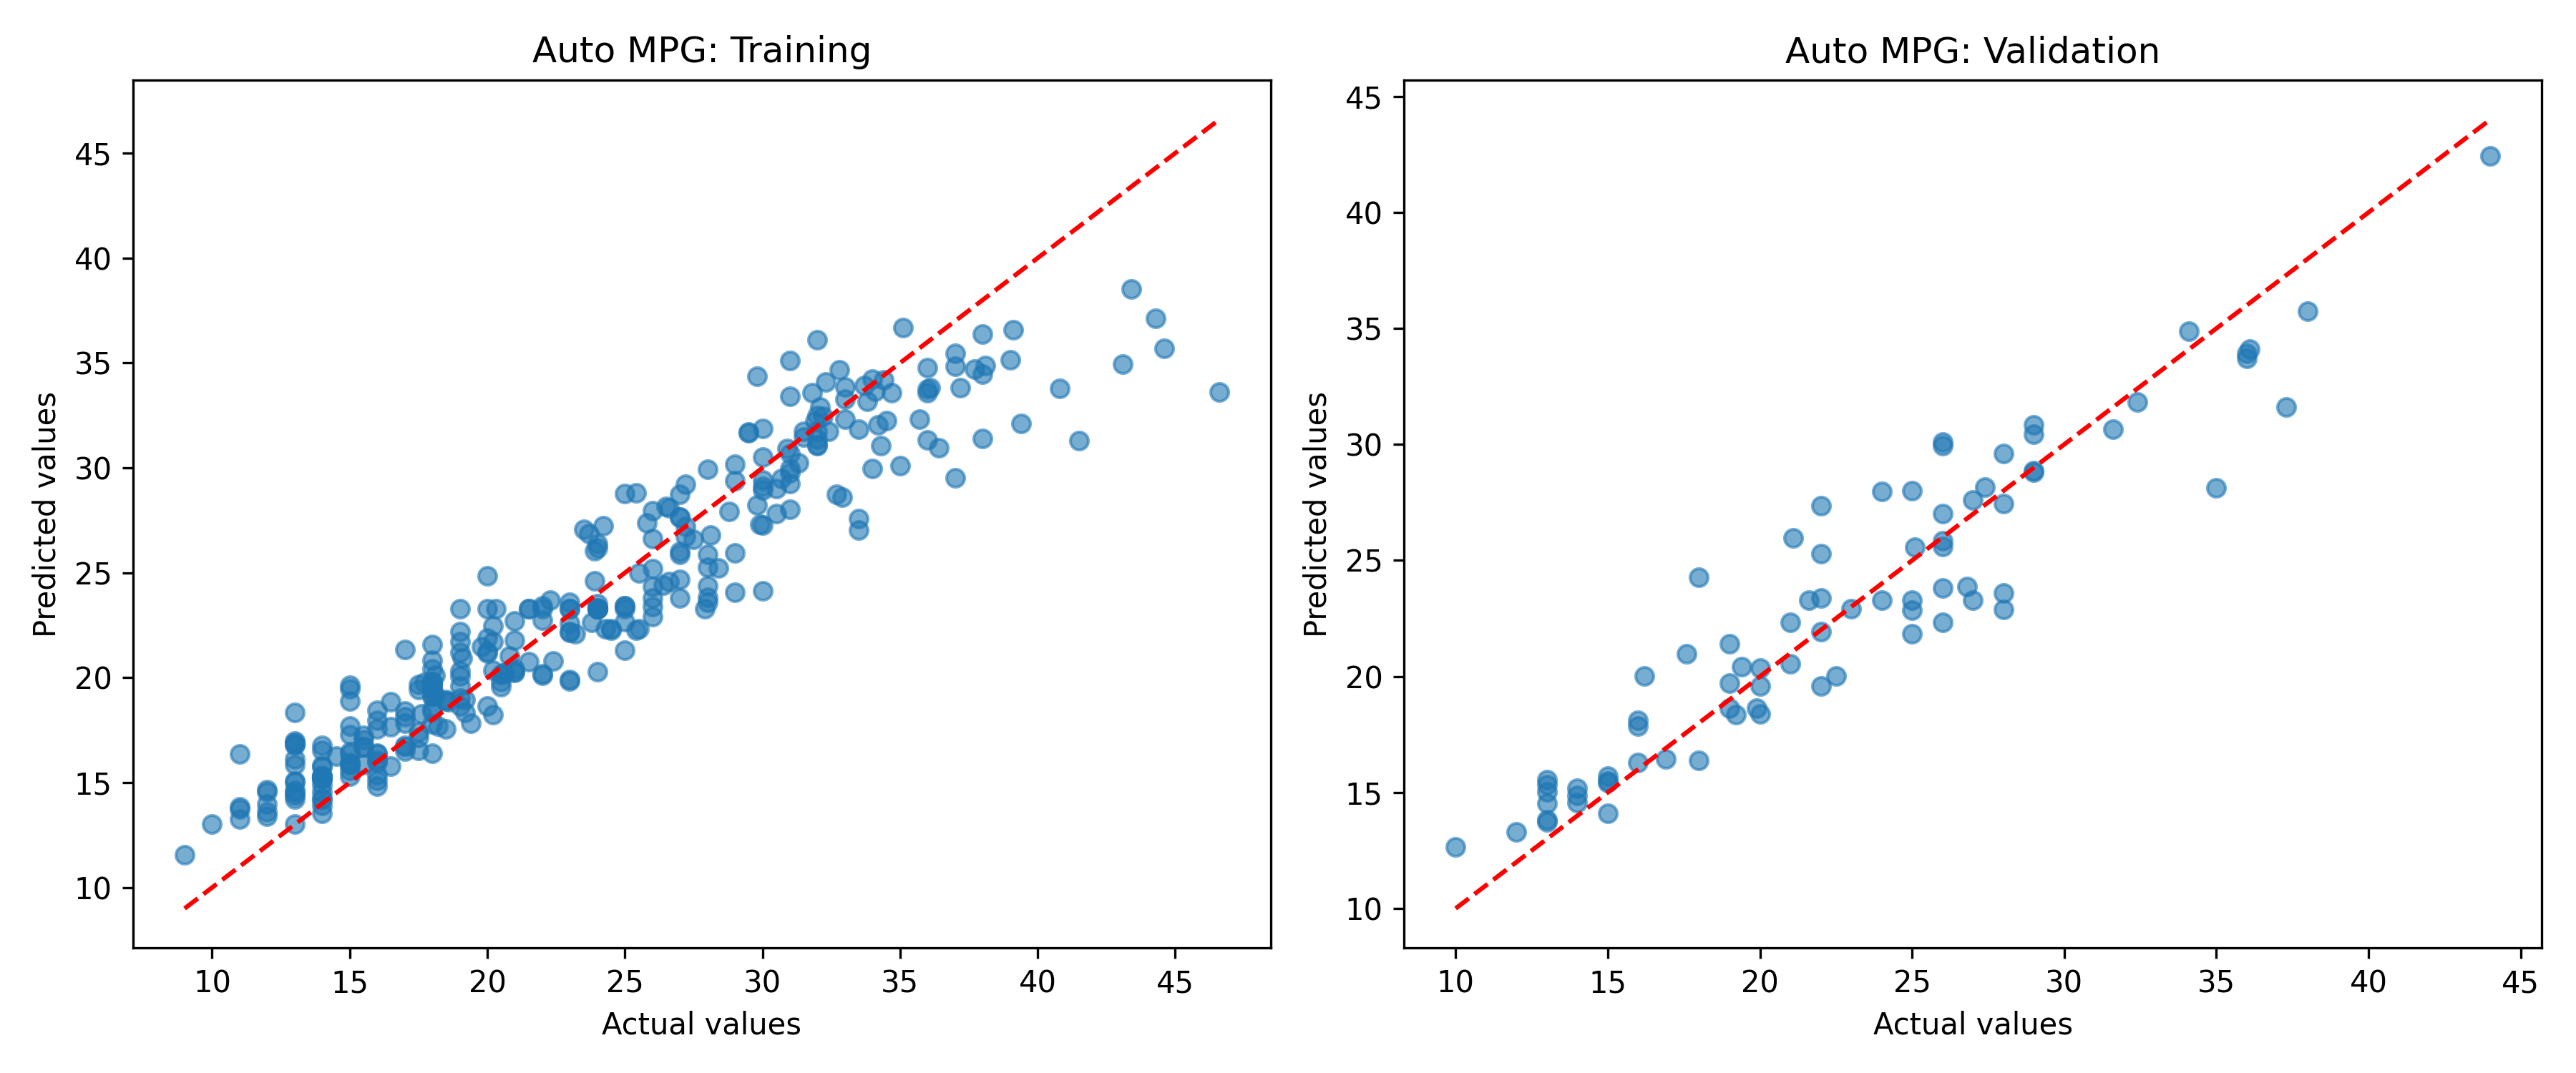
\includegraphics[width=0.85\linewidth]{5L/autompg_actual.png}
    \caption{PyTorch 5L Actual vs. Predicted Values for Auto MPG (Left: Training, Right: Validation)}
    \label{fig:pytorch5l_autompg}
\end{figure}
\begin{figure}[H]
    \centering
    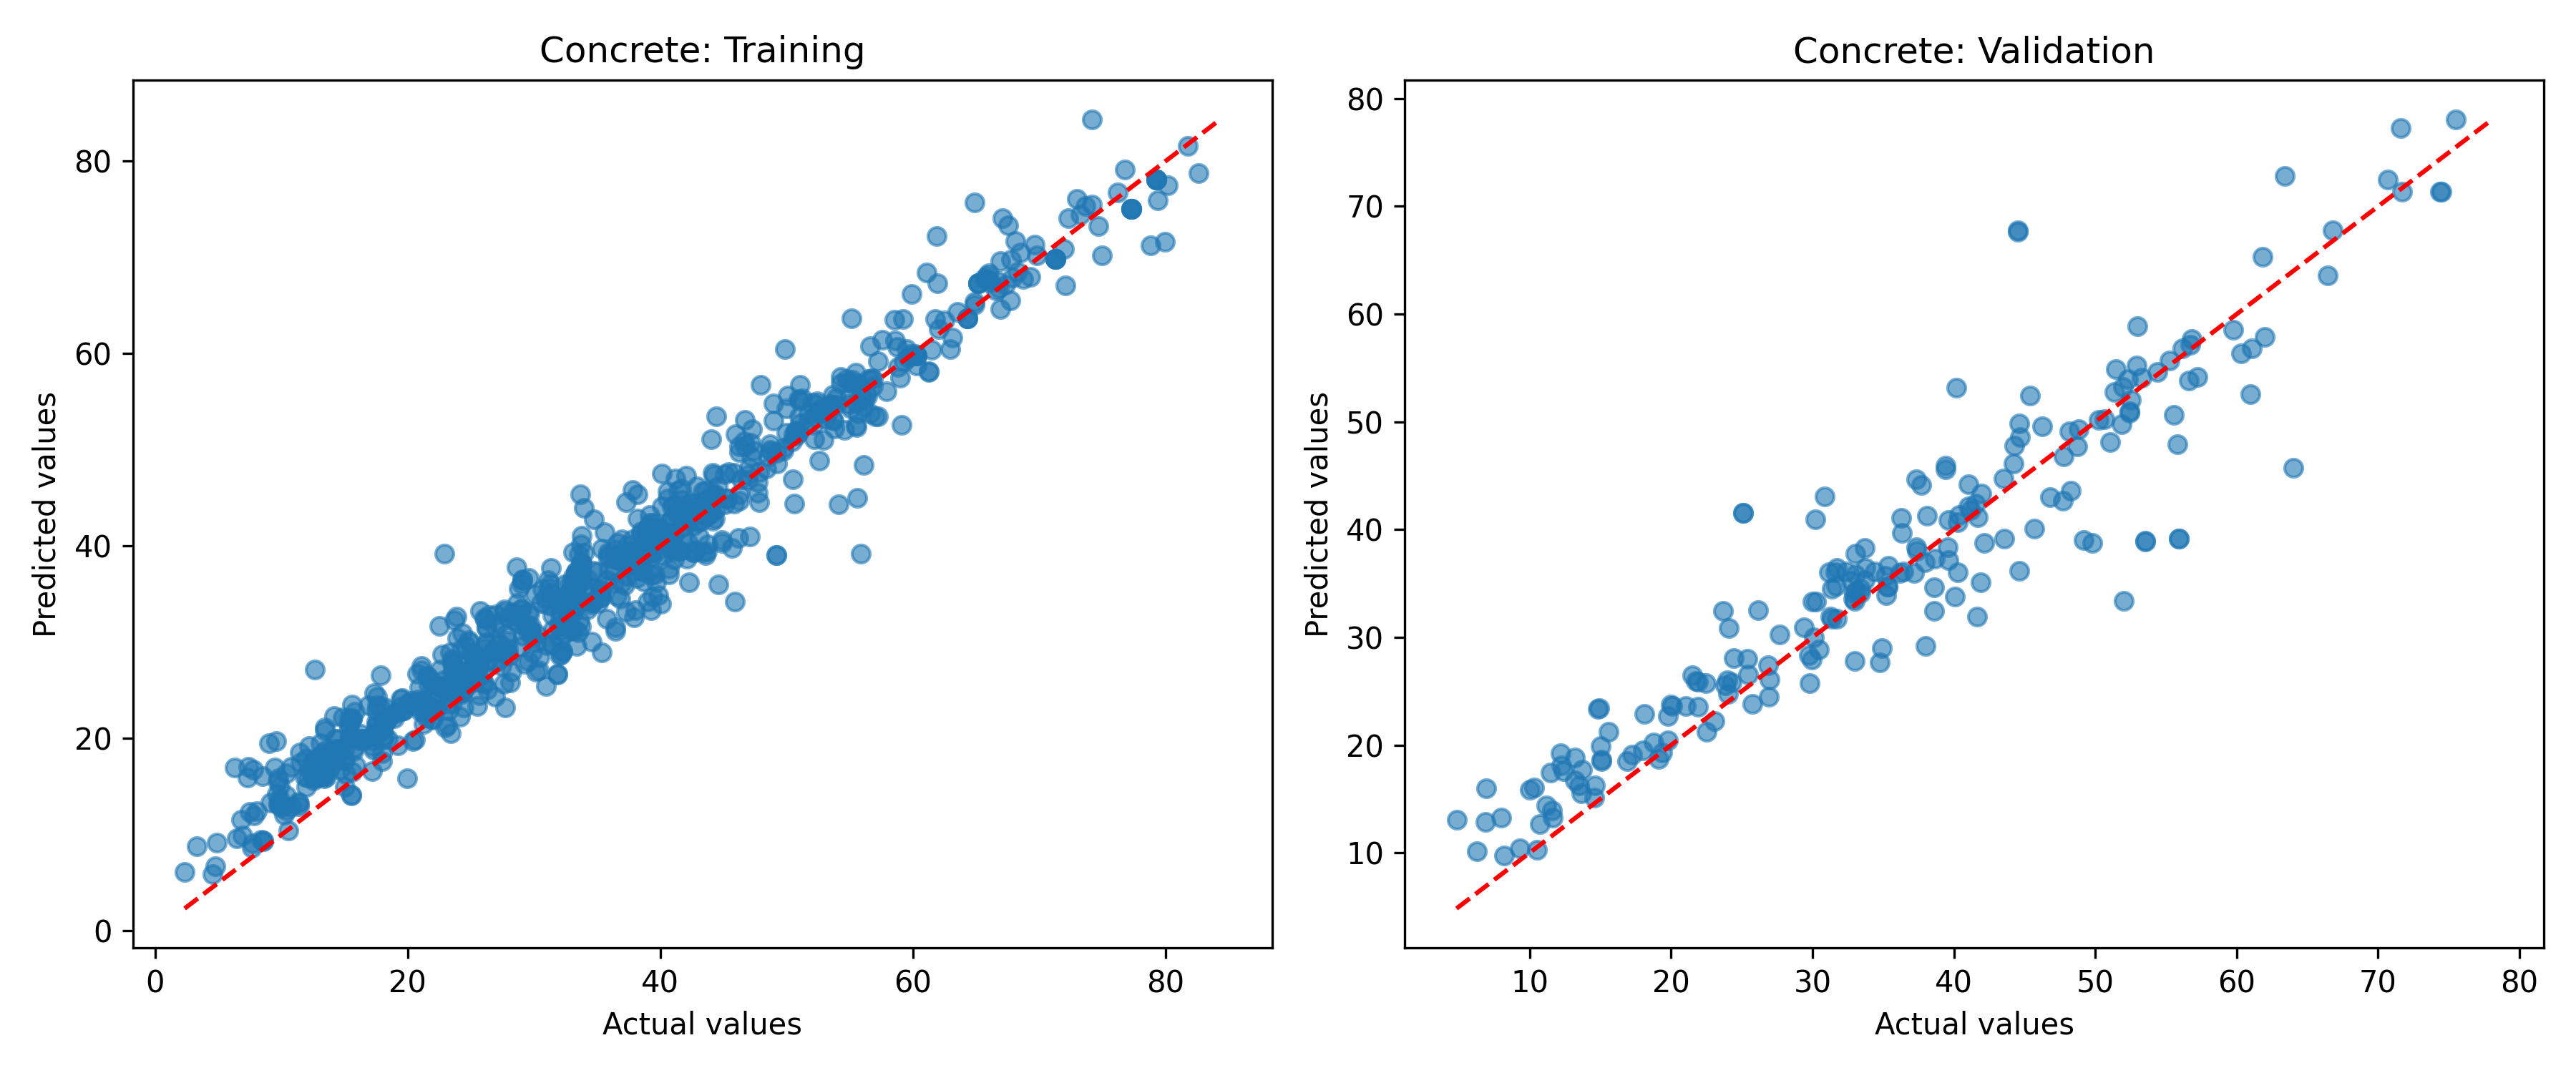
\includegraphics[width=0.85\linewidth]{5L/concrete_actual.png}
    \caption{PyTorch 5L Actual vs. Predicted Values for Concrete (Left: Training, Right: Validation)}
    \label{fig:pytorch5l_concrete}
\end{figure}

Figures \ref{fig:pytorch5l_airfoil}--\ref{fig:pytorch5l_concrete} show the actual vs predicted values, where the red dashed line represents perfect predictions. Most Airfoil points in both panels fall close to the diagonal across the full range of sound pressure levels. Auto MPG follows the diagonal with moderate spread in both panels. Concrete follows the diagonal closely on the training data, while the validation predictions show more spread, particularly at mid-range strengths.
\medskip
\begin{figure}[H]
    \centering

    \begin{minipage}{0.32\textwidth}
        \centering
        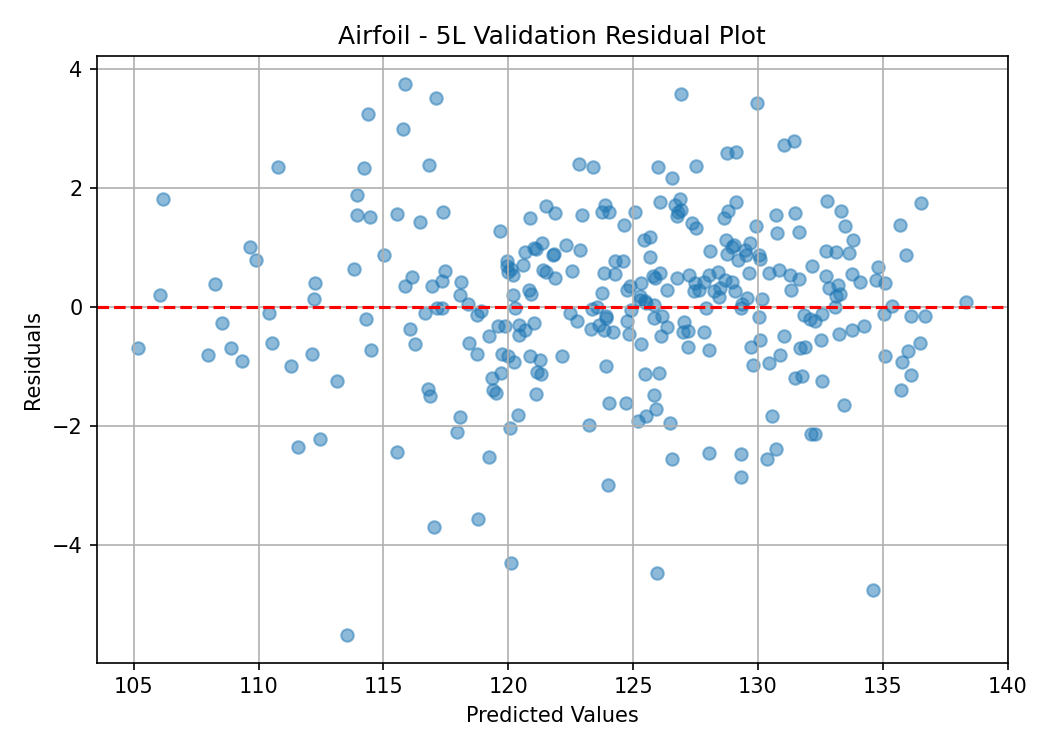
\includegraphics[width=\linewidth]{5L/airfoil_residual.png}
        \small (a) Airfoil
    \end{minipage}
    \hfill
    \begin{minipage}{0.32\textwidth}
        \centering
        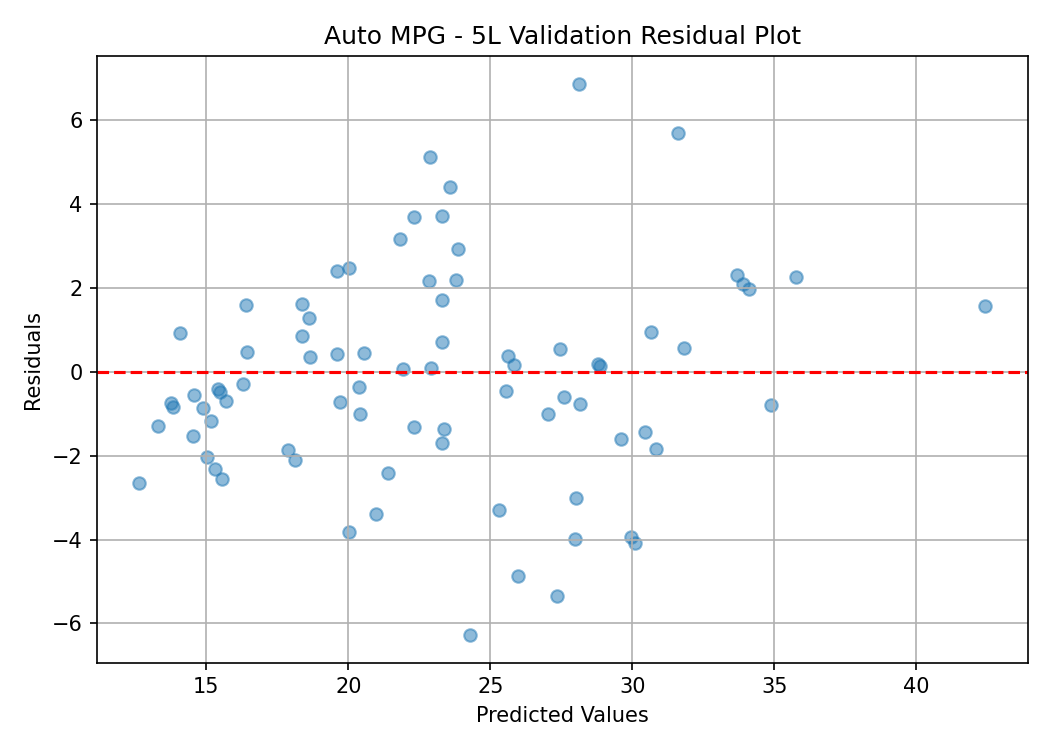
\includegraphics[width=\linewidth]{5L/autompg_residual.png}
        \small (b) Auto MPG
    \end{minipage}
    \hfill
    \begin{minipage}{0.32\textwidth}
        \centering
        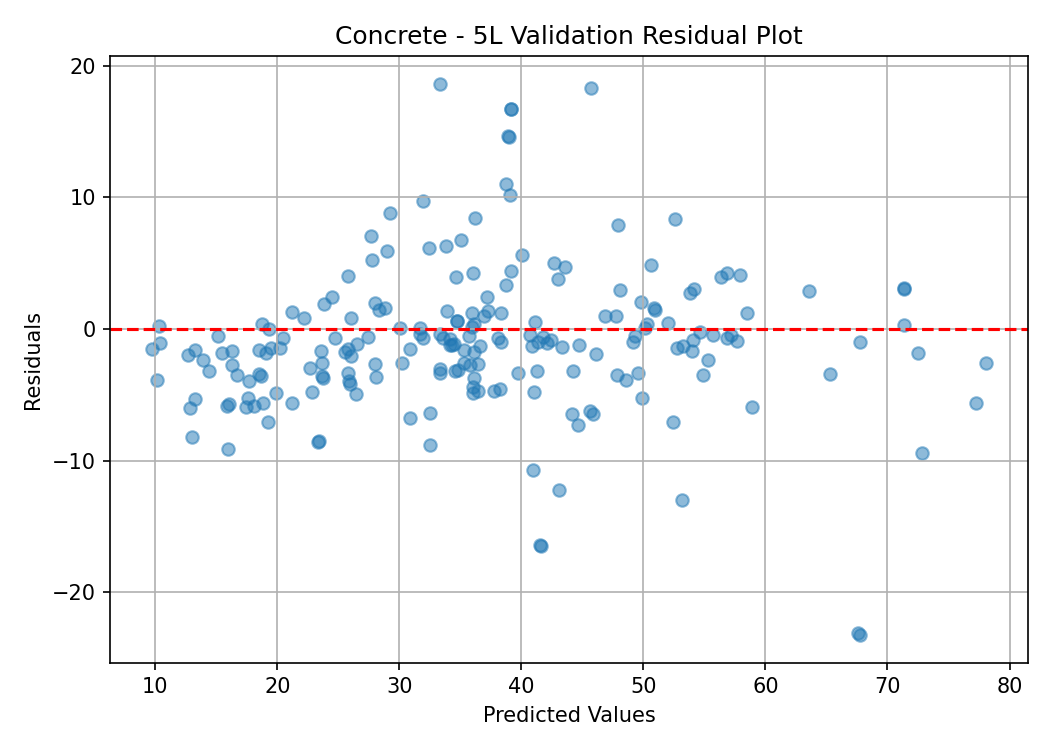
\includegraphics[width=\linewidth]{5L/concrete_residual.png}
        \small (c) Concrete
    \end{minipage}

    \caption{PyTorch 5L Neural Network Validation Residual Plots}
    \label{fig:pytorch5l_residual}
\end{figure}

Figure \ref{fig:pytorch5l_residual} shows the validation residuals against the predicted values. The Airfoil residuals are small (mostly within $\pm$3 dB) and show no clear pattern. The Auto MPG residuals stay within about $\pm$7 mpg and are spread fairly evenly around zero. The Concrete residuals are mostly within $\pm$10 MPa, but a few observations have much larger errors (up to about $-$23 MPa), which contribute to its higher validation MSE.

\subsubsection{Conclusion}
Overall, the 5L model performed best on Airfoil (validation R² of 0.9618) and showed the largest training--validation gap on Concrete. Its Airfoil and Concrete results are very close to those of the 4L model, so the third hidden layer did not provide a clear improvement over two hidden layers on these datasets. The Auto MPG result is the least stable across random seeds, so its single-seed validation R² should be interpreted with caution. RMSE values should be interpreted within each dataset because the response variables use different units and scales. These results describe the particular split and hyperparameter grid used in this experiment.

\section{Picked Architecture}
For the \textbf{Pick an Architecture} part of the project, a PyTorch network was designed to address the main weakness seen in the 4L and 5L models: overfitting on Concrete, where the training R² (0.95 to 0.96) was much higher than the validation R² (about 0.87). The picked architecture uses three hidden blocks with widths $(w, w, w/2)$, where each block applies a linear layer, \textbf{batch normalization}, an activation function, and \textbf{dropout}. Batch normalization normalizes the inputs of each layer within a mini-batch, which stabilizes training, and dropout randomly sets a fraction of the hidden nodes to zero during training, which discourages the network from relying on individual nodes. \textbf{Weight decay} (an L2 penalty on the weights in the Adam optimizer) was also tuned as an additional form of regularization. The output layer uses the identity activation for regression.
\medskip

The same 80/20 training-validation split, input and target standardization, inner 80/20 tuning split, and early-stopping procedure (maximum of 300 epochs, patience = 20) as the 4L and 5L models were used. The search covered 144 configurations per dataset: widths $w \in \{64, 128\}$; ReLU and SiLU activation functions (SiLU, $f(x) = x \cdot \mathrm{sigmoid}(x)$, is a smooth version of ReLU); dropout rates of 0, 0.1, and 0.2; weight decay of 0, $10^{-4}$, and $10^{-3}$; mini-batch sizes of 16 and 32; and learning rates of 0.001 and 0.005. The final model was retrained on the full training set for the best number of epochs found during tuning.

\subsection{Hyperparameter-Tuning Results}
\begin{table}[H]
    \centering
    \caption{Picked Architecture Hyperparameter Tuning Results}
    \label{tab:picked_hyperparameters}
    \small
    \resizebox{\textwidth}{!}{
    \begin{tabular}{lcccccccc}
        \hline
        \textbf{Dataset} & \textbf{Hidden Nodes} & \textbf{Activation} & \textbf{Dropout} & \textbf{Weight Decay} & \textbf{Learning Rate} & \textbf{Batch Size} & \textbf{Inner-Val. MSE} & \textbf{Best Epoch} \\
        \hline
        Airfoil  & (64, 64, 32)   & ReLU & 0.0 & $10^{-4}$ & 0.005 & 32 & 4.8545 & 75 \\
        Auto MPG & (64, 64, 32)   & SiLU & 0.0 & $10^{-4}$ & 0.001 & 16 & 5.6358 & 11 \\
        Concrete & (128, 128, 64) & ReLU & 0.0 & $10^{-3}$ & 0.001 & 32 & 19.2173 & 91 \\
        \hline
    \end{tabular}
    }
\end{table}

As shown in Table \ref{tab:picked_hyperparameters}, a dropout rate of 0 was selected for all three datasets, while a small amount of weight decay was selected for all three. Concrete selected the wider network (128 nodes) and the largest weight decay ($10^{-3}$), while Airfoil and Auto MPG selected the narrower network. ReLU was selected for Airfoil and Concrete, and SiLU for Auto MPG.
\medskip
\begin{figure}[H]
    \centering
    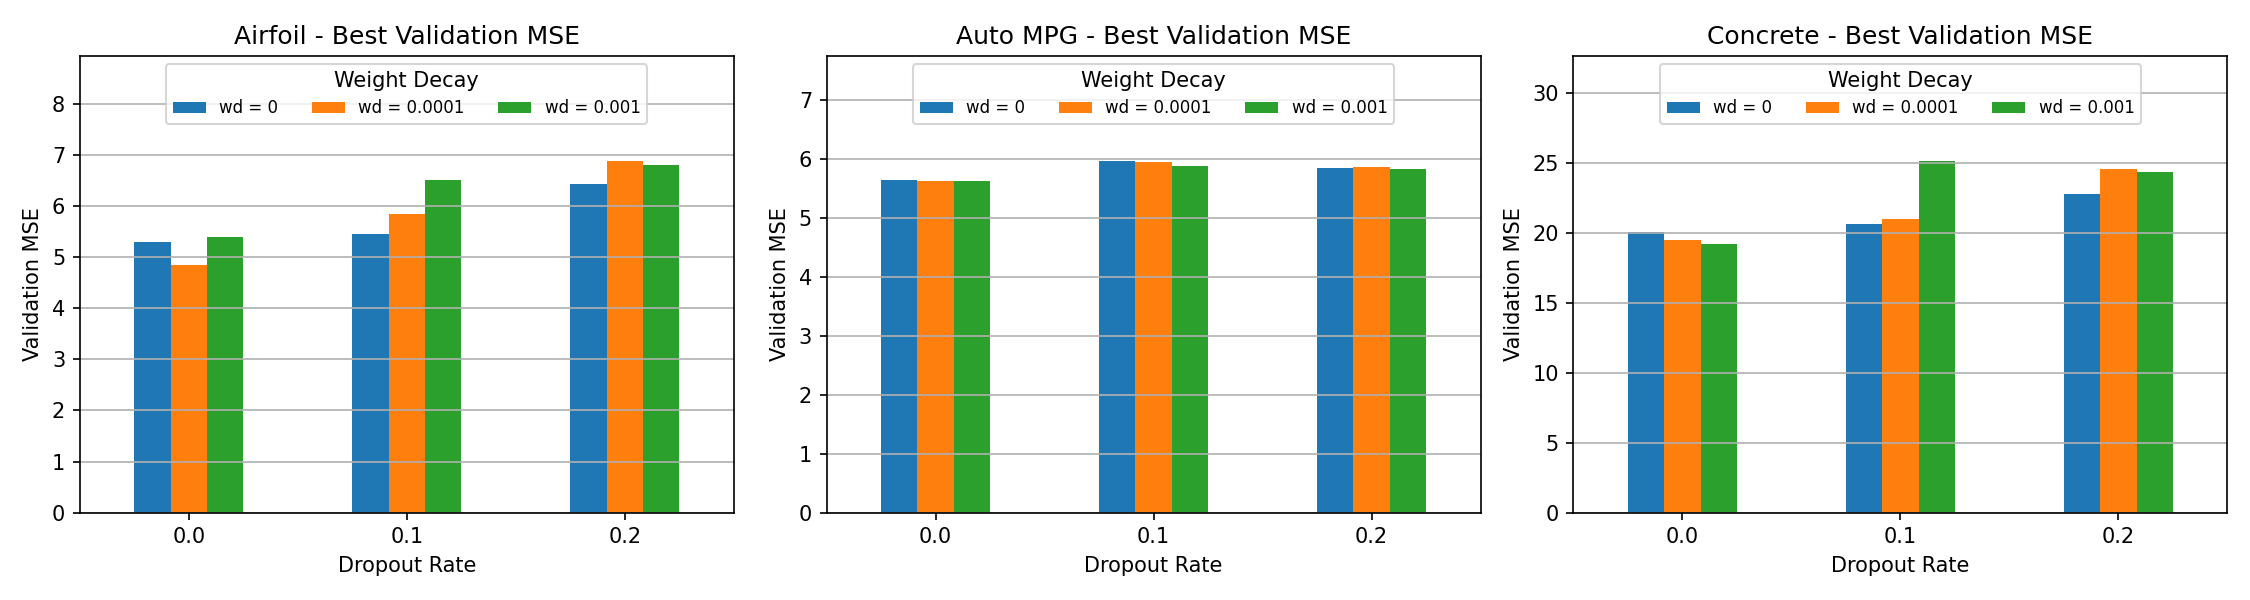
\includegraphics[width=\linewidth]{Custom/tuning_sensitivity.png}
    \caption{Picked Architecture Best Tuning Validation MSE by Dropout Rate and Weight Decay}
    \label{fig:picked_tuning}
\end{figure}

Figure \ref{fig:picked_tuning} shows the best tuning validation MSE for each dropout rate and weight decay. For Airfoil and Concrete, the validation MSE increases as the dropout rate increases, so dropout made the predictions worse rather than reducing overfitting. For Auto MPG, dropout and weight decay have almost no effect. These results suggest that, for these small tabular datasets, randomly removing hidden nodes removes useful information, while a small weight decay is a gentler and more effective form of regularization.

\subsection{Quality of Fit}
\begin{table}[H]
    \centering
    \caption{Picked Architecture Quality of Fit Results}
    \label{tab:picked_qof}
    \small
    \resizebox{\textwidth}{!}{
    \begin{tabular}{lcccccc}
        \hline
        \textbf{Dataset} & \textbf{Train $R^2$} & \textbf{Validation $R^2$} & \textbf{Train MSE} & \textbf{Validation MSE} & \textbf{Train RMSE} & \textbf{Validation RMSE} \\
        \hline
        Airfoil  & 0.8898 & 0.8688 & 5.1715 & 6.5710 & 2.2741 & 2.5634 \\
        Auto MPG & 0.8923 & 0.8717 & 6.7944 & 6.5488 & 2.6066 & 2.5591 \\
        Concrete & 0.9466 & 0.8677 & 15.1638 & 34.0992 & 3.8941 & 5.8394 \\
        \hline
    \end{tabular}
    }
\end{table}

As shown in Table \ref{tab:picked_qof}, the picked architecture achieved validation R² values of 0.8688 for Airfoil, 0.8717 for Auto MPG, and 0.8677 for Concrete. For Concrete, the training--validation R² gap decreased slightly compared with the 4L model (0.0790 versus 0.0932), but the validation R² did not improve (0.8677 versus 0.8691), so the added regularization did not solve the overfitting problem. For Airfoil, the validation R² is clearly lower than that of the 4L model (0.8688 versus 0.9643); batch normalization adds noise to each mini-batch, which appears to limit how precisely the network can fit the smooth Airfoil relationship. For Auto MPG, the picked architecture achieved a higher validation R² than the 4L model (0.8717 versus 0.8317).
\medskip

When the final models were retrained with five different seeds, the mean validation R² values were 0.8886 ($\pm$0.0220) for Airfoil, 0.8737 ($\pm$0.0082) for Auto MPG, and 0.8757 ($\pm$0.0026) for Concrete. The picked architecture was the most stable model for Auto MPG and Concrete (compared with standard deviations of 0.0255 and 0.0111 for the 4L model), which shows that batch normalization and weight decay make the results less sensitive to the random initialization, even when they do not increase the average accuracy.
\medskip
\begin{figure}[H]
    \centering

    \begin{minipage}{0.32\textwidth}
        \centering
        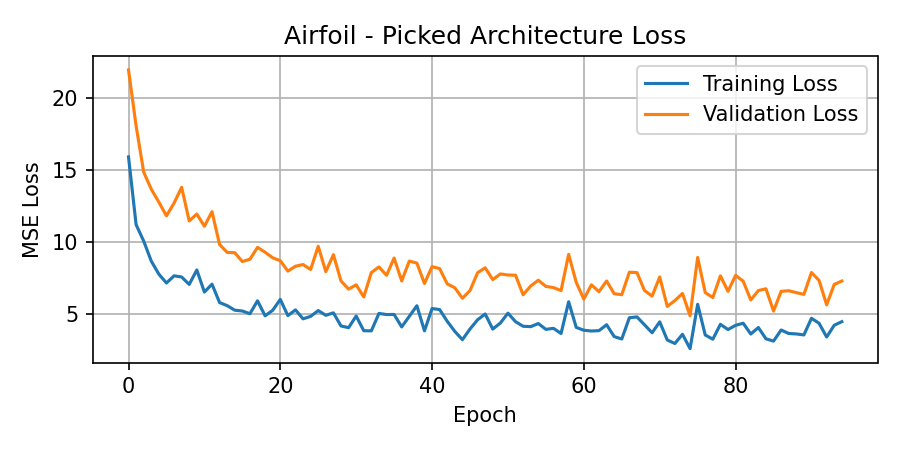
\includegraphics[width=\linewidth]{Custom/airfoil_loss.png}
        \small (a) Airfoil
    \end{minipage}
    \hfill
    \begin{minipage}{0.32\textwidth}
        \centering
        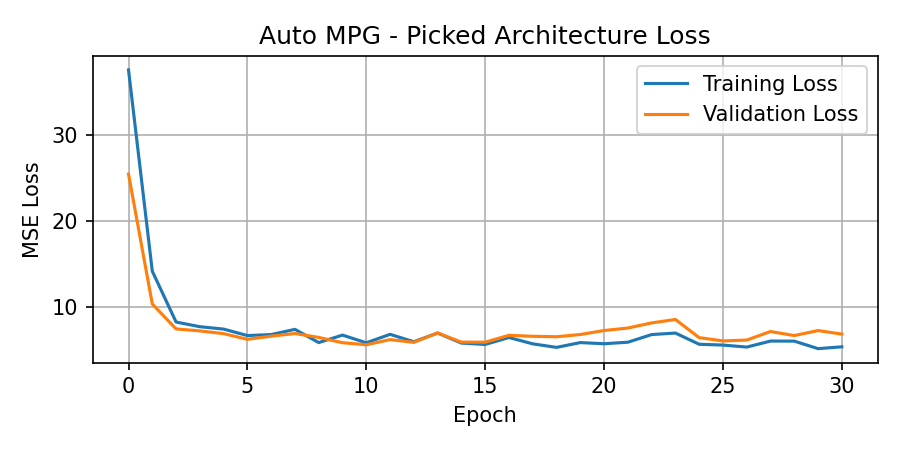
\includegraphics[width=\linewidth]{Custom/autompg_loss.png}
        \small (b) Auto MPG
    \end{minipage}
    \hfill
    \begin{minipage}{0.32\textwidth}
        \centering
        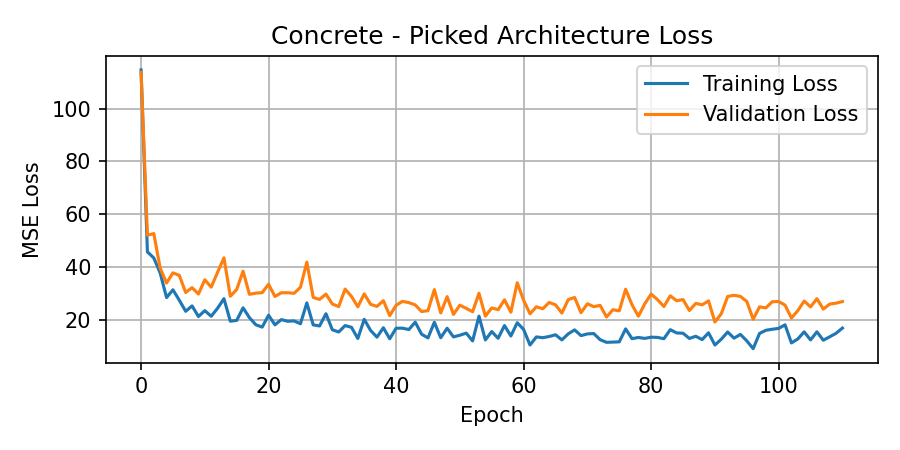
\includegraphics[width=\linewidth]{Custom/concrete_loss.png}
        \small (c) Concrete
    \end{minipage}

    \caption{Picked Architecture Training and Validation Loss vs. Epoch (Tuning Run, Selected Configuration)}
    \label{fig:picked_loss}
\end{figure}

Figure \ref{fig:picked_loss} shows the training and inner-validation loss for the selected configuration of each dataset. All three datasets drop sharply in the first few epochs. Auto MPG has the smoothest curves of all the PyTorch models, with almost no gap between training and validation loss, consistent with its low variability across seeds. Airfoil and Concrete keep a visible gap between training and validation loss and are noisier, which reflects the mini-batch noise added by batch normalization.
\medskip
\begin{figure}[H]
    \centering

    \begin{minipage}{0.32\textwidth}
        \centering
        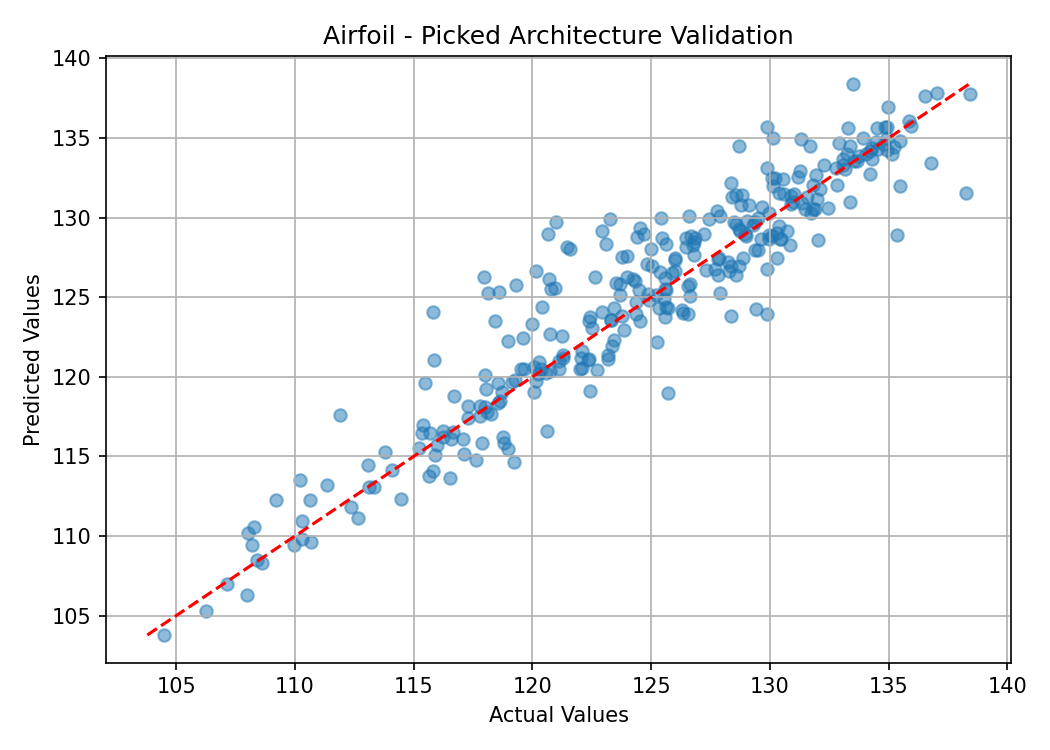
\includegraphics[width=\linewidth]{Custom/airfoil_actual.png}
        \small (a) Airfoil
    \end{minipage}
    \hfill
    \begin{minipage}{0.32\textwidth}
        \centering
        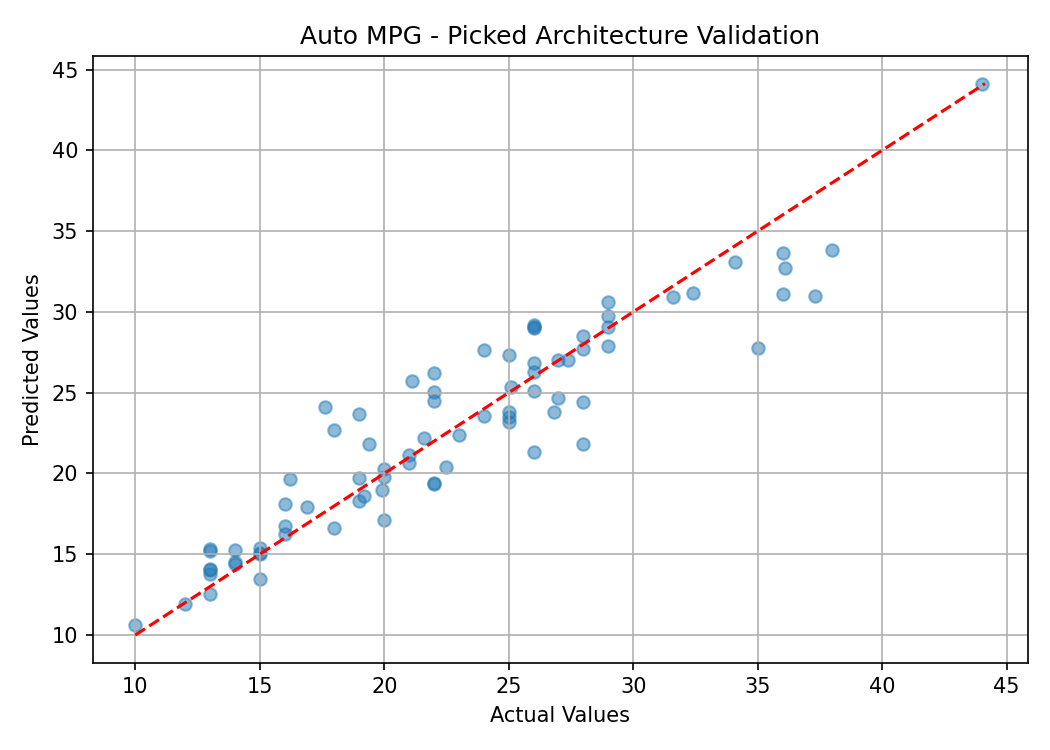
\includegraphics[width=\linewidth]{Custom/autompg_actual.png}
        \small (b) Auto MPG
    \end{minipage}
    \hfill
    \begin{minipage}{0.32\textwidth}
        \centering
        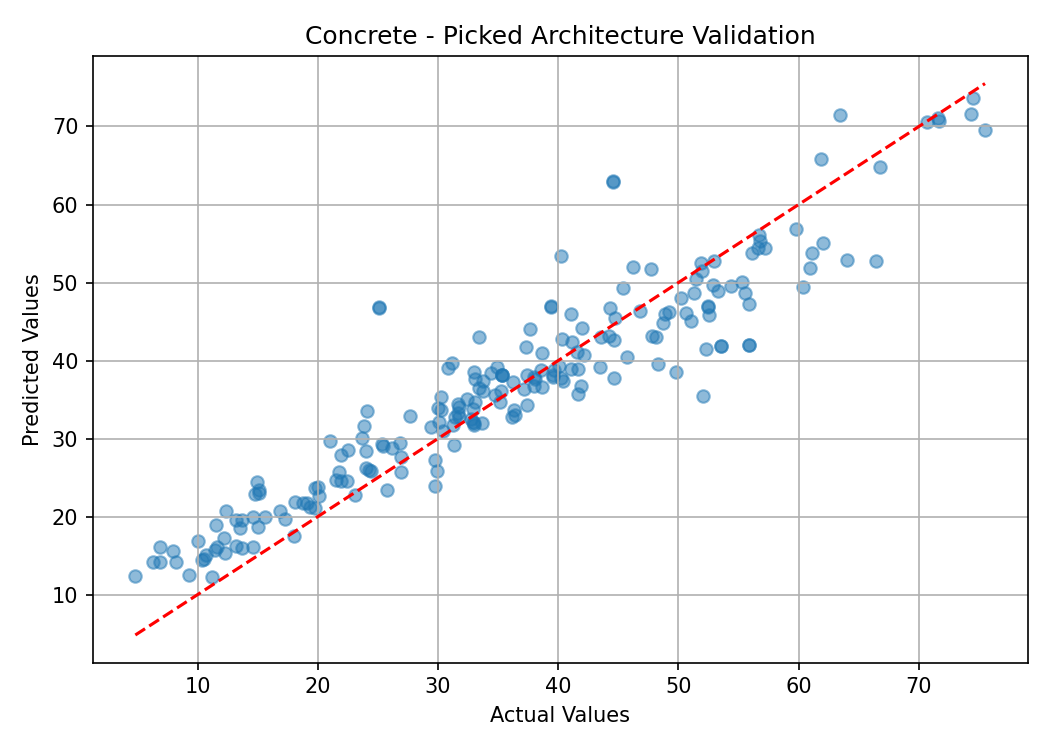
\includegraphics[width=\linewidth]{Custom/concrete_actual.png}
        \small (c) Concrete
    \end{minipage}

    \caption{Picked Architecture Validation Actual vs. Predicted Values}
    \label{fig:picked_actual}
\end{figure}

\begin{figure}[H]
    \centering

    \begin{minipage}{0.32\textwidth}
        \centering
        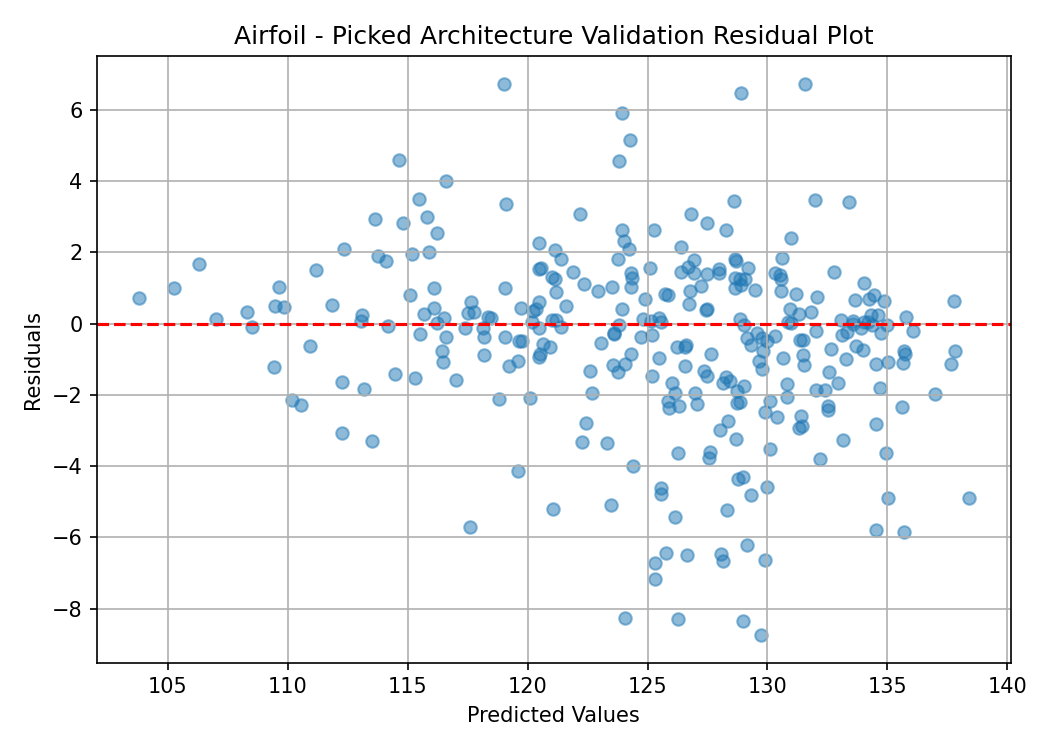
\includegraphics[width=\linewidth]{Custom/airfoil_residual.png}
        \small (a) Airfoil
    \end{minipage}
    \hfill
    \begin{minipage}{0.32\textwidth}
        \centering
        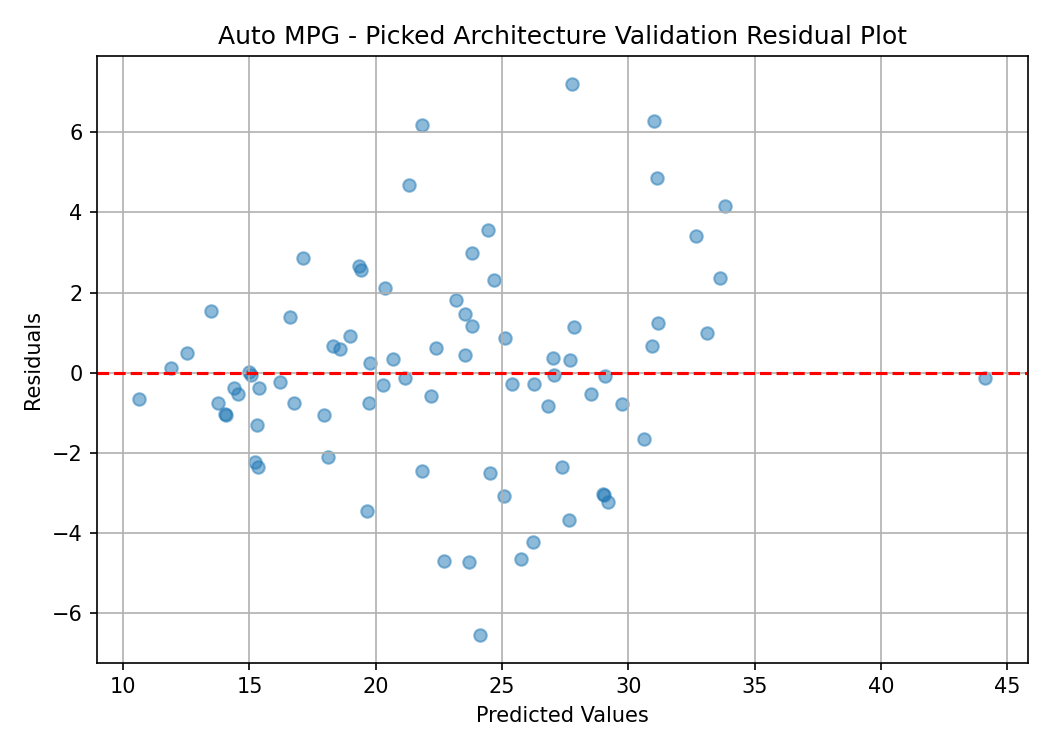
\includegraphics[width=\linewidth]{Custom/autompg_residual.png}
        \small (b) Auto MPG
    \end{minipage}
    \hfill
    \begin{minipage}{0.32\textwidth}
        \centering
        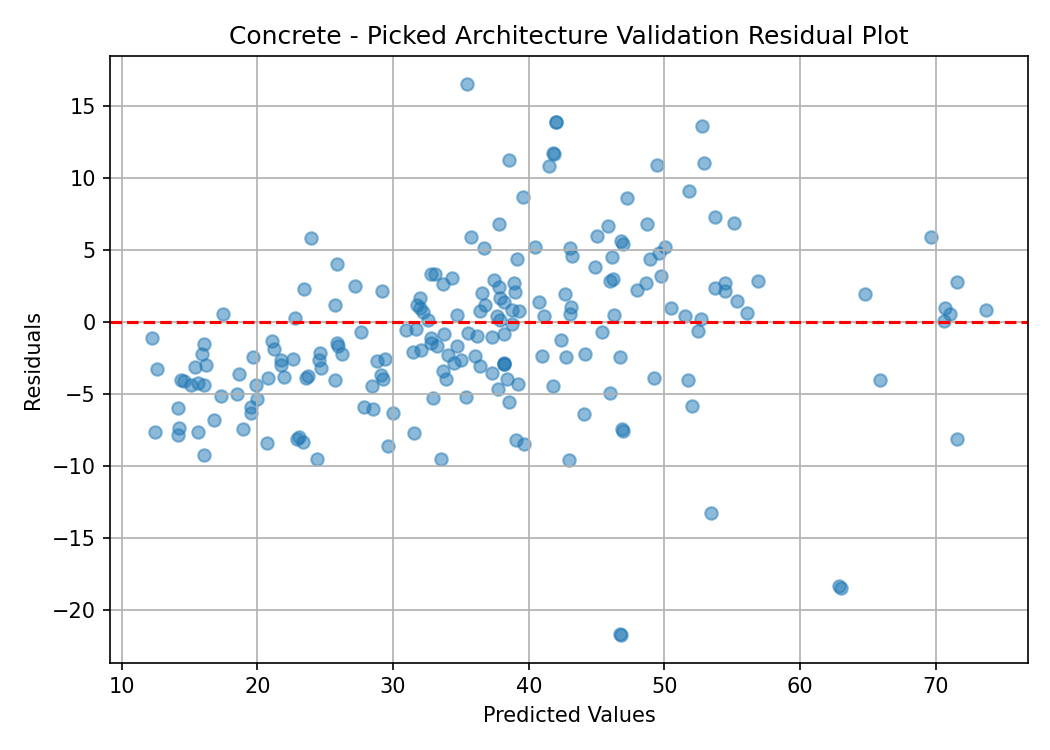
\includegraphics[width=\linewidth]{Custom/concrete_residual.png}
        \small (c) Concrete
    \end{minipage}

    \caption{Picked Architecture Validation Residual Plots}
    \label{fig:picked_residual}
\end{figure}

Figures \ref{fig:picked_actual} and \ref{fig:picked_residual} show the validation actual vs predicted values and residuals. Auto MPG follows the diagonal closely, and its residuals are spread fairly evenly around zero within about $\pm$7 mpg. The Airfoil residuals are more widely spread than for the 4L model, and many of the largest errors are negative for predicted values between about 120 and 135 dB, meaning that the model tends to overpredict sound pressure in that range, which is consistent with its lower validation R². The Concrete residuals are mostly within $\pm$10 MPa, with a few large errors near $-$20 MPa, similar to the 4L and 5L models.

\subsection{Conclusion}
The picked architecture shows that adding regularization does not automatically improve predictive accuracy. Dropout consistently hurt performance on these small tabular datasets, and batch normalization reduced the accuracy on Airfoil. However, the architecture produced the most stable Auto MPG and Concrete results across random seeds and the best average Auto MPG validation R² of all the PyTorch models (0.8737). Overall, it is a reasonable choice for the small, noisy Auto MPG dataset, while the simpler 4L network remains the better choice for Airfoil.

\section{Comparison of Models and Discussion}
\begin{table}[H]
    \centering
    \caption{Validation $R^2$ for All Models and Datasets (Single Run)}
    \label{tab:all_models}
    \begin{tabular}{llccc}
        \hline
        \textbf{Model} & \textbf{Software} & \textbf{Airfoil} & \textbf{Auto MPG} & \textbf{Concrete} \\
        \hline
        2L                  & ScalaTion & 0.4880 & 0.8035 & 0.6076 \\
        2L                  & PyTorch   & 0.5528 & 0.7829 & 0.6236 \\
        3L                  & ScalaTion & 0.9287 & 0.8479 & \textbf{0.8986} \\
        3L                  & PyTorch   & 0.9072 & 0.8526 & 0.8923 \\
        4L                  & PyTorch   & \textbf{0.9643} & 0.8317 & 0.8691 \\
        5L                  & PyTorch   & 0.9618 & \textbf{0.8813} & 0.8723 \\
        Picked Architecture & PyTorch   & 0.8688 & 0.8717 & 0.8677 \\
        \hline
    \end{tabular}
\end{table}

\begin{table}[H]
    \centering
    \caption{Mean Validation $R^2$ ($\pm$ Standard Deviation) over Five Random Seeds for the PyTorch Models with Hidden Layers}
    \label{tab:all_models_seeds}
    \begin{tabular}{lccc}
        \hline
        \textbf{Model} & \textbf{Airfoil} & \textbf{Auto MPG} & \textbf{Concrete} \\
        \hline
        3L                  & 0.9026 ($\pm$0.0055) & 0.8277 ($\pm$0.0197) & 0.8746 ($\pm$0.0169) \\
        4L                  & \textbf{0.9610} ($\pm$0.0082) & 0.8525 ($\pm$0.0255) & 0.8738 ($\pm$0.0111) \\
        5L                  & 0.9506 ($\pm$0.0074) & 0.8269 ($\pm$0.0472) & \textbf{0.8795} ($\pm$0.0122) \\
        Picked Architecture & 0.8886 ($\pm$0.0220) & \textbf{0.8737} ($\pm$0.0082) & 0.8757 ($\pm$0.0026) \\
        \hline
    \end{tabular}
\end{table}

Table \ref{tab:all_models} summarizes the validation R² of every model on every dataset, and Table \ref{tab:all_models_seeds} reports the average over five random seeds for the PyTorch models with hidden layers. All PyTorch models use the same training and validation observations, while the ScalaTion models use a different random split, so comparisons between ScalaTion and PyTorch should be interpreted with caution.
\medskip

\textbf{Effect of hidden layers.} The largest improvement for every dataset came from adding the first hidden layer. Moving from 2L to 3L raised the validation R² from about 0.49--0.55 to 0.91--0.93 for Airfoil and from about 0.61--0.62 to about 0.89--0.90 for Concrete, while Auto MPG improved only from about 0.78--0.80 to 0.85. This confirms that Airfoil and Concrete have strongly nonlinear relationships that a linear 2L model cannot capture, while Auto MPG is much closer to linear.
\medskip

\textbf{Effect of depth.} Additional hidden layers gave diminishing returns. Airfoil benefited from a second hidden layer (mean validation R² of 0.9026 for 3L versus 0.9610 for 4L), but a third hidden layer (5L) did not improve it further. For Concrete, all models with hidden layers reached a very similar validation R² (about 0.87--0.90), and the five-seed means of the PyTorch models differ by less than 0.006, so depth had almost no effect. All of these Concrete models also show a clear training--validation gap, which suggests that the remaining error is limited by the size and noise of the dataset rather than by the network architecture. For Auto MPG, the differences between models are of the same size as the variation across random seeds (up to $\pm$0.047 for 5L), so no architecture is clearly better than the others on this small dataset; the picked architecture had the highest and most stable average.
\medskip

\textbf{Best model for each dataset.} Based on both the single-run and five-seed results, the 4L network is the best model for Airfoil (validation R² of 0.9643, five-seed mean of 0.9610). For Auto MPG, the picked architecture gives the best and most stable average (0.8737 $\pm$ 0.0082), although the 5L network had the highest single-run value. For Concrete, the ScalaTion 3L network had the highest single-run validation R² (0.8986), and among the PyTorch models the 3L network had the highest single-run value (0.8923), while the five-seed averages of all PyTorch models are nearly identical; the simpler 3L network is therefore a reasonable choice for Concrete.
\medskip

\textbf{Software comparison.} ScalaTion and PyTorch produced similar results for the same architectures. For 2L, both are close to linear regression, and for 3L the validation R² values differ by at most about 0.02. The remaining differences are likely due to the different random splits, optimizer settings, number of epochs, and hyperparameter grids rather than the software itself.

\subsection{Conclusion}
Across the three datasets, neural networks with at least one hidden layer clearly outperformed the 2L network, with the largest gains on the nonlinear Airfoil and Concrete datasets. Adding more hidden layers helped Airfoil up to two hidden layers but gave little or no further improvement for Auto MPG and Concrete. The picked architecture showed that regularization techniques such as dropout and batch normalization do not always improve accuracy on small tabular datasets, although they can make the results more stable. Standardizing the target, using early stopping, and checking several random seeds were all important for obtaining reliable results. These conclusions are based on a single 80/20 split per dataset, so cross-validation or additional splits would be needed to confirm them.

\end{document}
